\documentclass[italian, a4paper, 12pt]{article}

\usepackage[utf8]{inputenc}
\usepackage[T1]{fontenc}
\usepackage{babel}

\usepackage[left=25mm, top=20mm, right=25mm, bottom=20mm]{geometry}
\renewcommand{\baselinestretch}{1.5}

\usepackage{float}

%%% font & looks %%%
\usepackage{mathpazo}
%\usepackage{palatino}
%\usepackage{kpfonts}
%\usepackage{times}
%\usepackage{charter}
%\usepackage{utopia}

% list of fonts available here - http://www.tug.dk/FontCatalogue/
% and here - https://www.sharelatex.com/learn/Font_typefaces

\usepackage{microtype}

\usepackage[parfill]{parskip}

\usepackage{bm}
\usepackage[labelfont=bf,font={small,it}]{caption}
\usepackage[usenames,dvipsnames,svgnames,table]{xcolor}

\usepackage{newtxtext}
\usepackage{newtxmath}

%%% boxes %%%
\usepackage{framed}
%\setlength\FrameSep{0.5em}

% math
%\usepackage{amsmath}
\usepackage{amssymb}
%\usepackage{amsthm}
\usepackage{wasysym}
%\usepackage{siunitx}

% graphics
\usepackage{multirow}
\usepackage[section]{placeins}
\usepackage{graphicx}
\usepackage{epstopdf}
\usepackage{pgfplots}
  \pgfplotsset{compat=newest}
  %% the following commands are needed for some matlab2tikz features
  \usetikzlibrary{plotmarks}
  \usetikzlibrary{arrows.meta}
  \usepgfplotslibrary{patchplots}
  \usepackage{grffile}
  \usepackage{amsmath}

\usepackage{pdfpages}

% extra
\usepackage{todonotes} %\todo{ note } , \listoftodos
\usepackage{blindtext}
\usepackage{lipsum}
\usepackage{tikz}
\usetikzlibrary{patterns}
\usetikzlibrary{decorations.pathreplacing,angles,quotes}
\usepackage{chemformula}
\usepackage{textcomp}
\usepackage{subcaption}

% better tables
\usepackage{booktabs}

%%% links %%%
\usepackage{hyperref}
\hypersetup{
        linktocpage,
        colorlinks,
    citecolor=black,
    filecolor=black,
    linkcolor=black,
    urlcolor=black
}

\usepackage[framed,numbered]{matlab-prettifier}
\tikzset{
  font={\fontsize{9pt}{12}\selectfont}}

\usepackage[sorting=none]{biblatex}
\addbibresource{report.bib}

%%% references %%%
\usepackage[noabbrev,capitalize,nameinlink]{cleveref}

% new commands
\newcommand{\horline}{\rule{1\linewidth}{0.9pt}}
\newcommand{\curl}{\nabla \times}
\renewcommand{\div}{\nabla \cdot}
\newcommand{\laplac}{\nabla^2}
\newcommand{\grad}{\nabla}

%\usepackage{mathspec}

%\newcommand{\mathbbm}[1]{\text{\usefont{U}{bbm}{m}{n}#1}} % from mathbbm.sty
%\newcommand{\indi}[1]{\operatorname{\mathbbm{1}}\left[#1\right]}
\newcommand{\mathbbm}[1]{\text{\usefont{U}{bbm}{m}{n}#1}} % from mathbbm.sty

\newcommand{\E}[1]{\operatorname{E}\left[#1\right]}
\newcommand{\EnB}{\E{\#_B}}

\newtheorem{p}{\\[5mm] \large Problem}
\newenvironment{s}{%\small%
        \begin{trivlist} \item \textbf{Solution}. }{%
\end{trivlist}}%
\begin{document}
\begin{center}
        %\horline\\
        \Large Wireless Systems And Networks\\
        \huge \textbf{Project: Unequal Error Protection}\\[3mm]
        \begin{framed}
                \Large \textbf{Workgroup} \\[2mm]
                \normalsize \textbf{Costa} Roberto -- \textbf{Zanol} Riccardo
        \end{framed}
        %\horline
\end{center}
\FloatBarrier
% Total max 15 pages
\section*{Sommario} % Max 10 lines
La tesina si prefigge di implementare un protocollo per trasmettere flussi video attraverso una rete non completamente affidabile, utilizzando un codice di correzione degli errori a fontana, il quale regola la ridondanza aggiunta ai dati in base alla loro importanza e in base alle necessità di ritrasmissione dei ricevitori.
Verrà analizzata la correttezza della trasmissione (in termini di Bit Error Rate) al variare della Bit Error Rate del canale. Verranno inoltre analizzate la complessità computazionale di codifica e decodifica e il tempo ad esse associato, al variare della ridondanza aggiunta.\\
Il progetto è stato realizzato usando C++ e Python.
\newpage
\section{Introduzione} % Max 1 page
Spesso, al giorno d'oggi, la qualità delle connessioni tra i dispositivi di una rete è variabile, anche, ad esempio, a causa di meccanismi di condivisione di risorse adattativi, finalizzati al rispetto di vincoli variabili di throughput per un numero variabile di utenti. Variabile è anche l'insieme di dispositivi connessi alla rete e il link budget di ogni dispositivo. Quando è necessario trasmettere un flusso video a un insieme di utenti, la qualità del video, in questo tipo di rete, dev'essere necessariamente variabile in base alla banda disponibile ad ogni utente. Un protocollo che si presta al multicast video attraverso connessioni eterogenee è l'estensione Scalable Video Coding (SVC) del protocollo H.264/MPEG-4 AVC \cite{svc}. Tale protocollo, infatti, permette di codificare il video una sola volta per tutti gli utenti, separando il file originale in un numero arbitrario di stream, la cui composizione garantisce alta fedeltà di ricostruzione del flusso video originale, ma non è indispensabile avere tutti le componenti per ricostruire un video a qualità inferiore.\\
Per trasmettere un flusso di dati attraverso un canale variabile e non completamente affidabile, garantendo la qualità del servizio, è utile aggiungere ridondanza all'informazione inviata. Il rapporto tra il messaggio con ridondanza aggiunta e il messaggio originale è chiamato rate del codice di correzione degli errori.
I codici a fontana \cite{fcsurvey, rossifc} presentano due caratteristiche notevoli, rispetto ad altri codici di correzione degli errori:
\begin{itemize}
\item Bassa complessità computazionale per la codifica e per la decodifica
\item Assenza di un code rate fisso.
\end{itemize}
I codici a fontana possono essere usati per proteggere allo stesso modo tutti i dati da trasmettere, caso in cui la ridondanza aggiunta dipende solo dalle condizioni del canale (EEP, equal error protection), oppure si possono proteggere maggiormente i dati più sensibili (UEP, unequal error protection \cite{uep}), caso in cui la ridondanza aggiunta dipende anche dall'importanza del dato.\\
Il vantaggio dato dalla possibilità di aggiungere una quantità arbitraria di ridondanza, oltre che nel proteggere meglio i dati più sensibili, risiede anche nella possibilità di sfruttare un canale che ha un comportamento variabile nel tempo e ignoto a priori: la quantità di ridondanza aggiunta può crescere al peggiorare delle condizioni del canale, a differenza di un codice a rate fisso che comporta uno spreco di banda se il canale è in buone condizioni, o insufficiente protezione se il canale non è in buone condizioni.
\section{Approccio tecnico}
\subsection{Obbiettivi} % Max 5 lines
La finalità del progetto è estendere il paper \cite{uep}, in cui è proposto un algoritmo per l'UEP basato sui codici a fontana, testando l'algoritmo di trasmissione con protezione non uniforme nel caso di un canale che introduce errori.
%
Considerando sia il caso di errori indipendenti che il caso di errori correlati, questo progetto vuole dimostrare che il protocollo di protezione non uniforme è utile ed efficiente anche in condizioni non error-free.
\subsection{Scenario} % Max 20 lines
Lo scenario considerato rappresentato in figura~\ref{fig:UDP}. Un
server trasmette un video H264 a un client segmentandolo in pacchetti
di lunghezza costante e divisi in due classi di priorità. I pacchetti
sono aggregati in blocchi con una struttura fissata (cioè contengono
sempre lo stesso numero di pacchetti per ogni classe di priorità). I
blocchi sono poi codificati utilizzando l'algoritmo proposto in
\cite{uep}, a un livello di overhead fissato e inviati dentro
pacchetti UDP al client.
%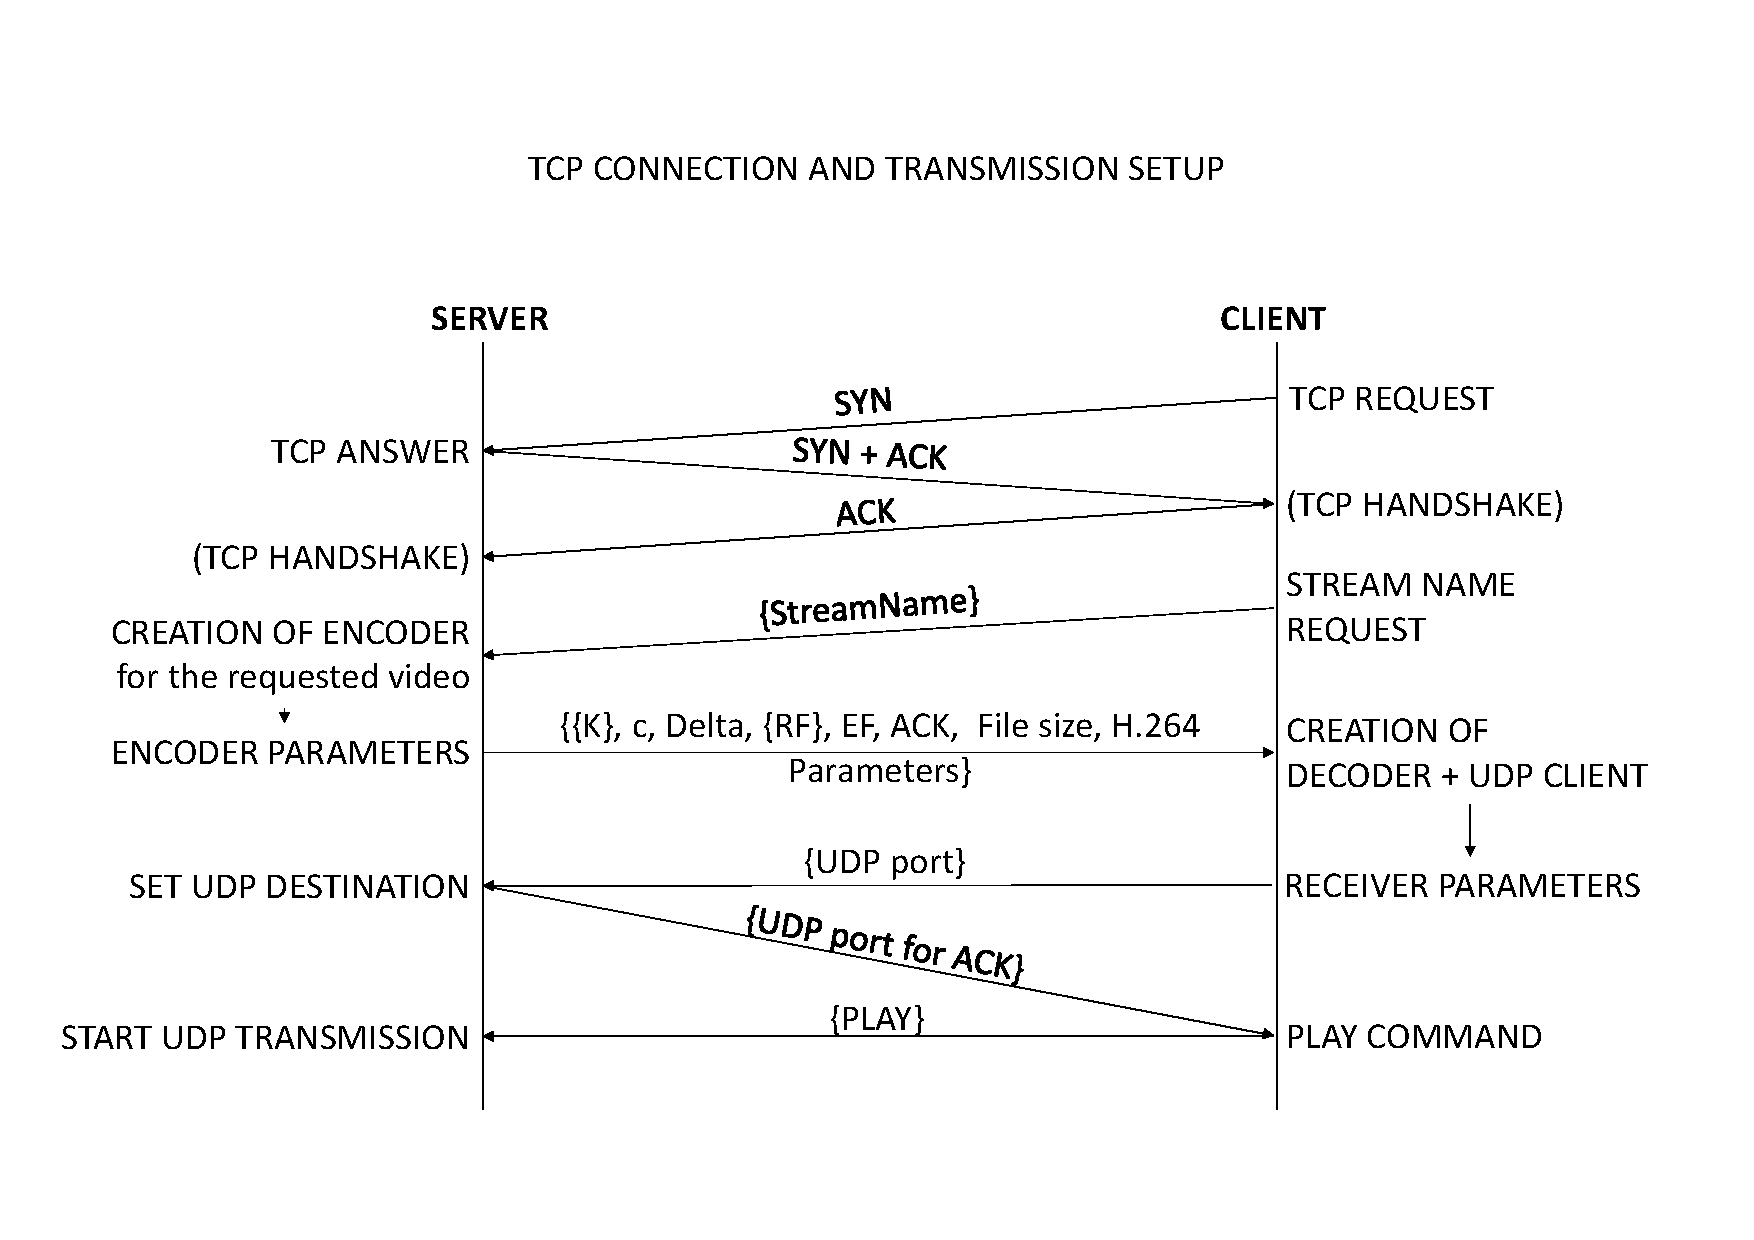
\includegraphics[trim=0cm 8cm 0cm 7cm, width=1.00\textwidth]{TCP.pdf}
%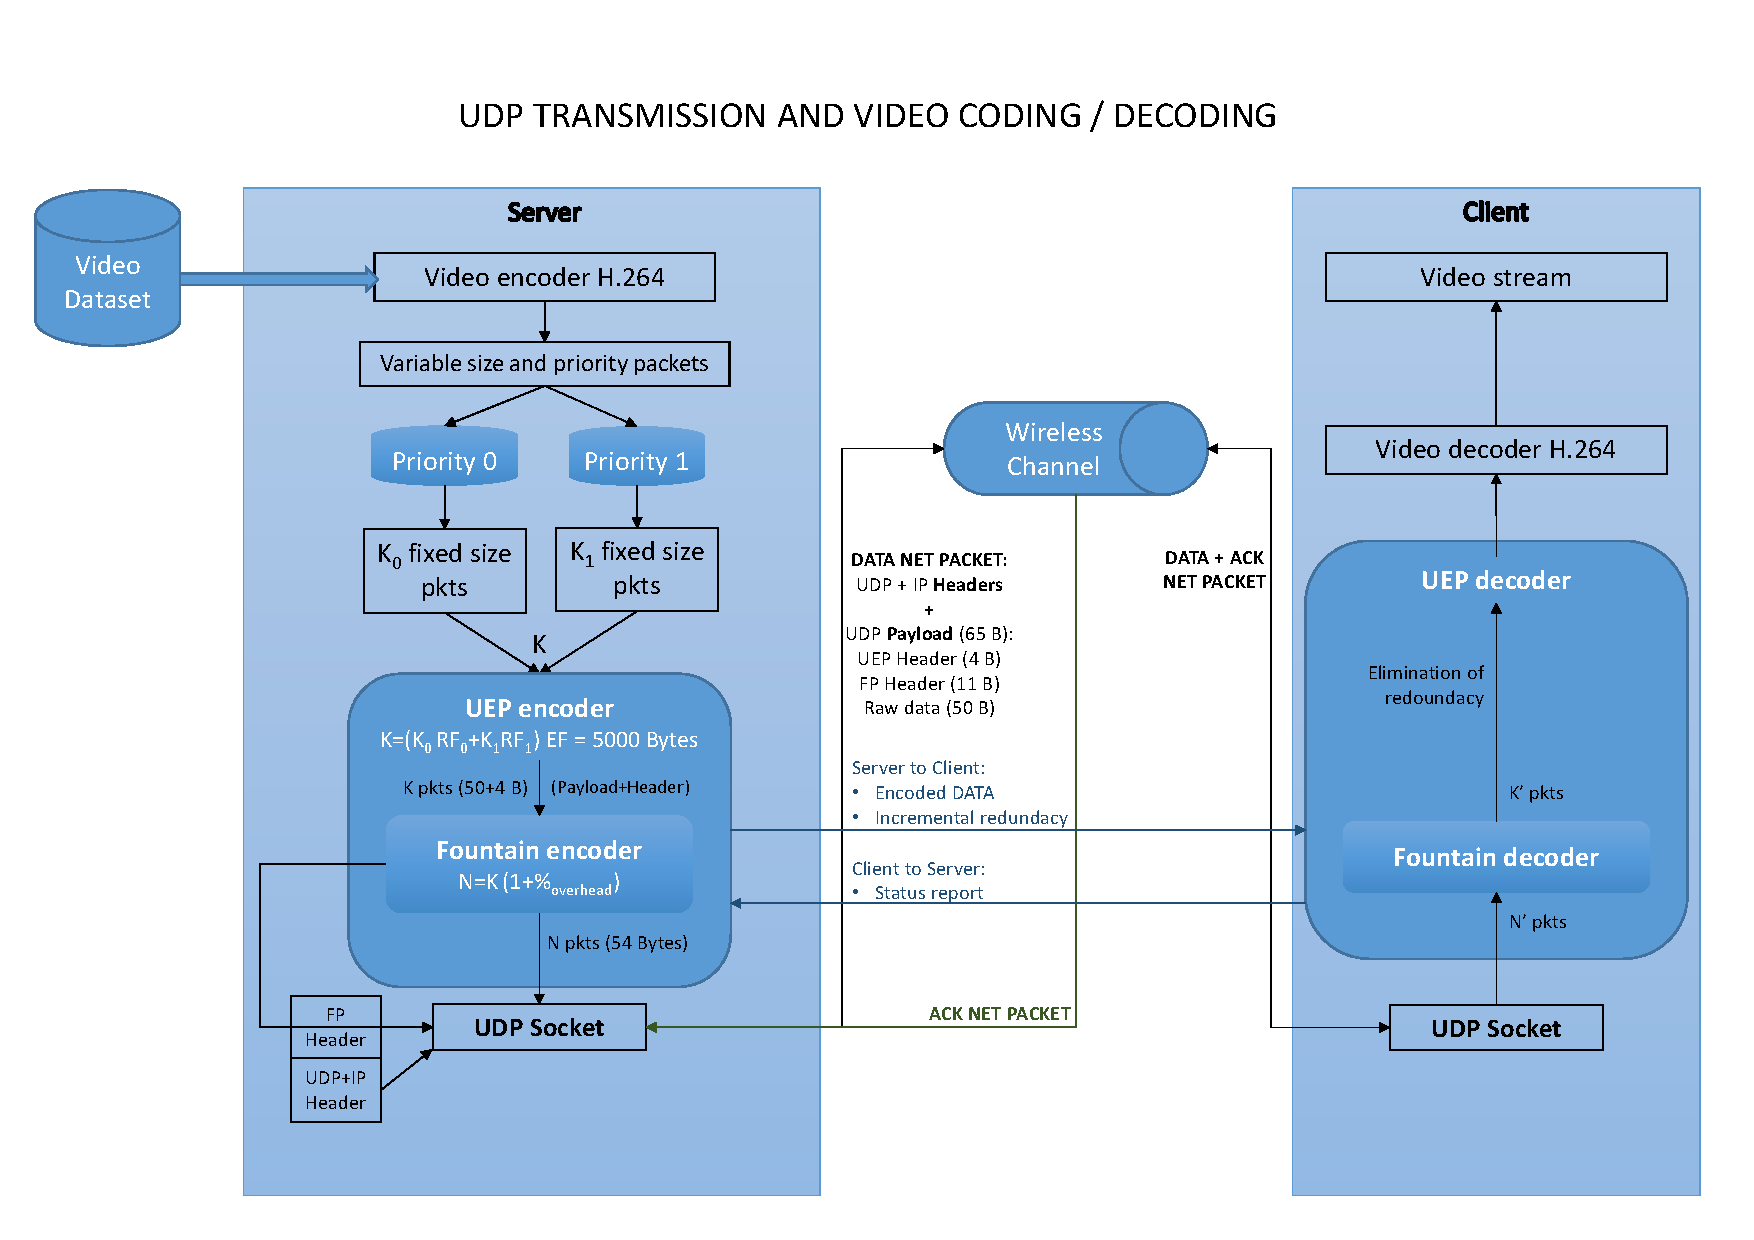
\includegraphics[width=180mm]{UDP.pdf}
%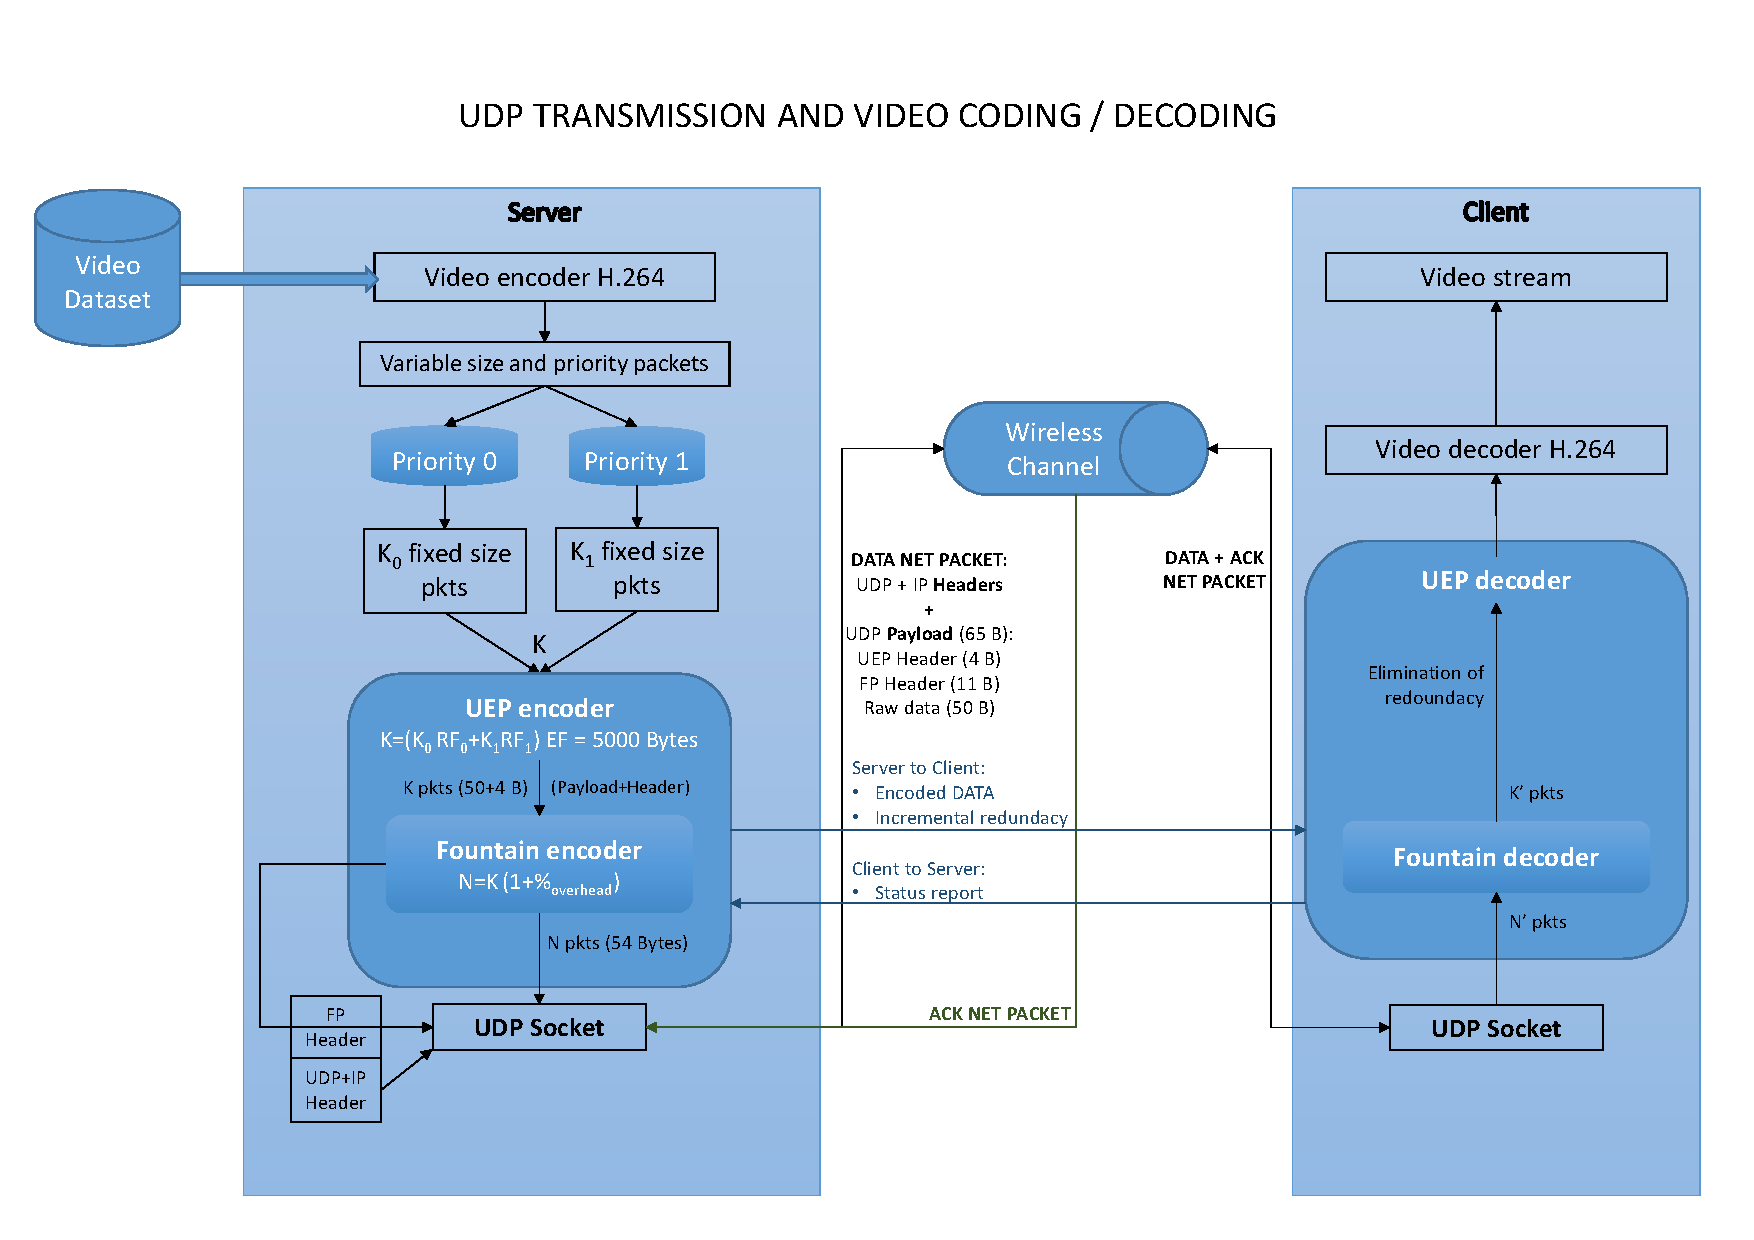
\includepdf[pages={1}]{UDP.pdf}
%\begin{figure}[htbp]
\begin{figure}[H]
    \centering
        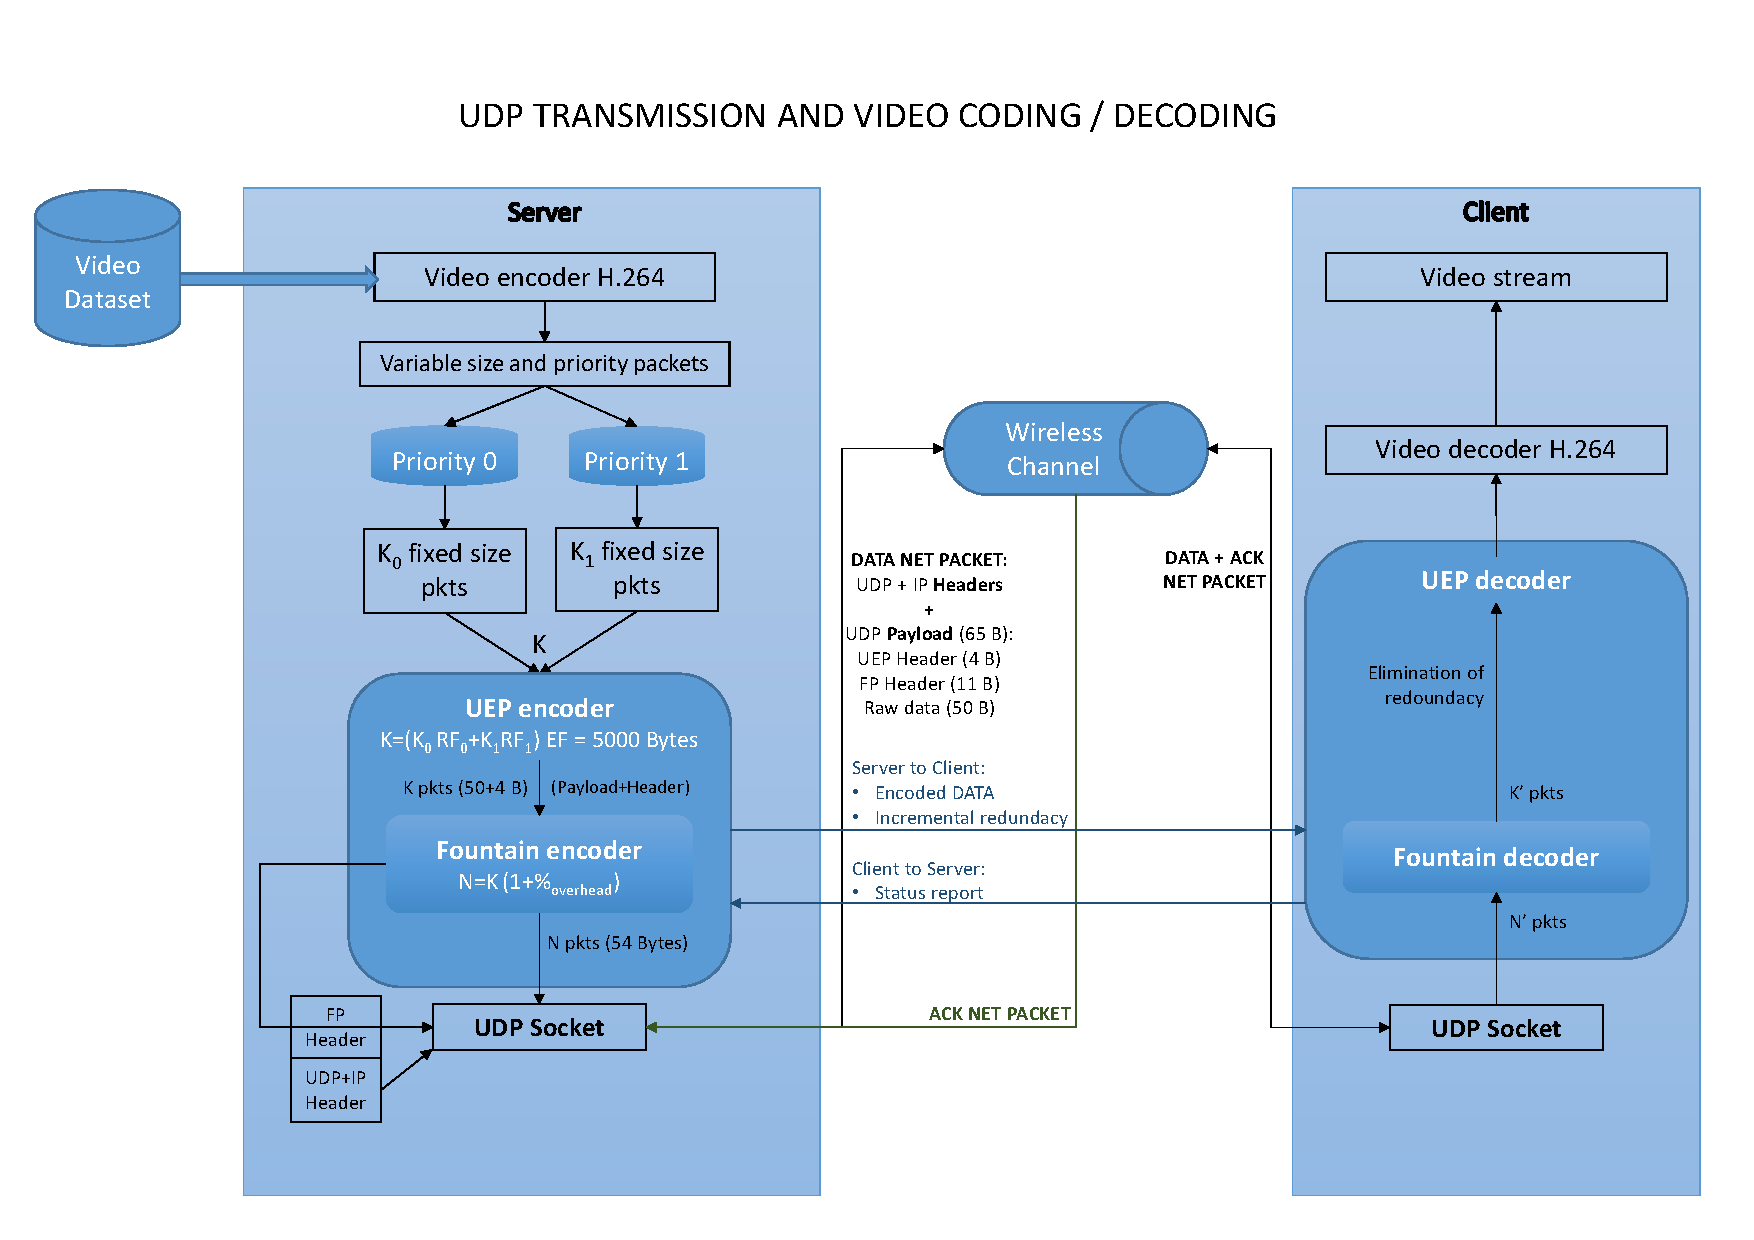
\includegraphics[clip, trim=0cm 1cm 0cm 1cm, width=1.00\textwidth]{UDP.pdf}
    \caption{Video stream encoding / decoding and transmission}
    \label{fig:UDP}
\end{figure}
\begin{figure}[H]
    \centering
        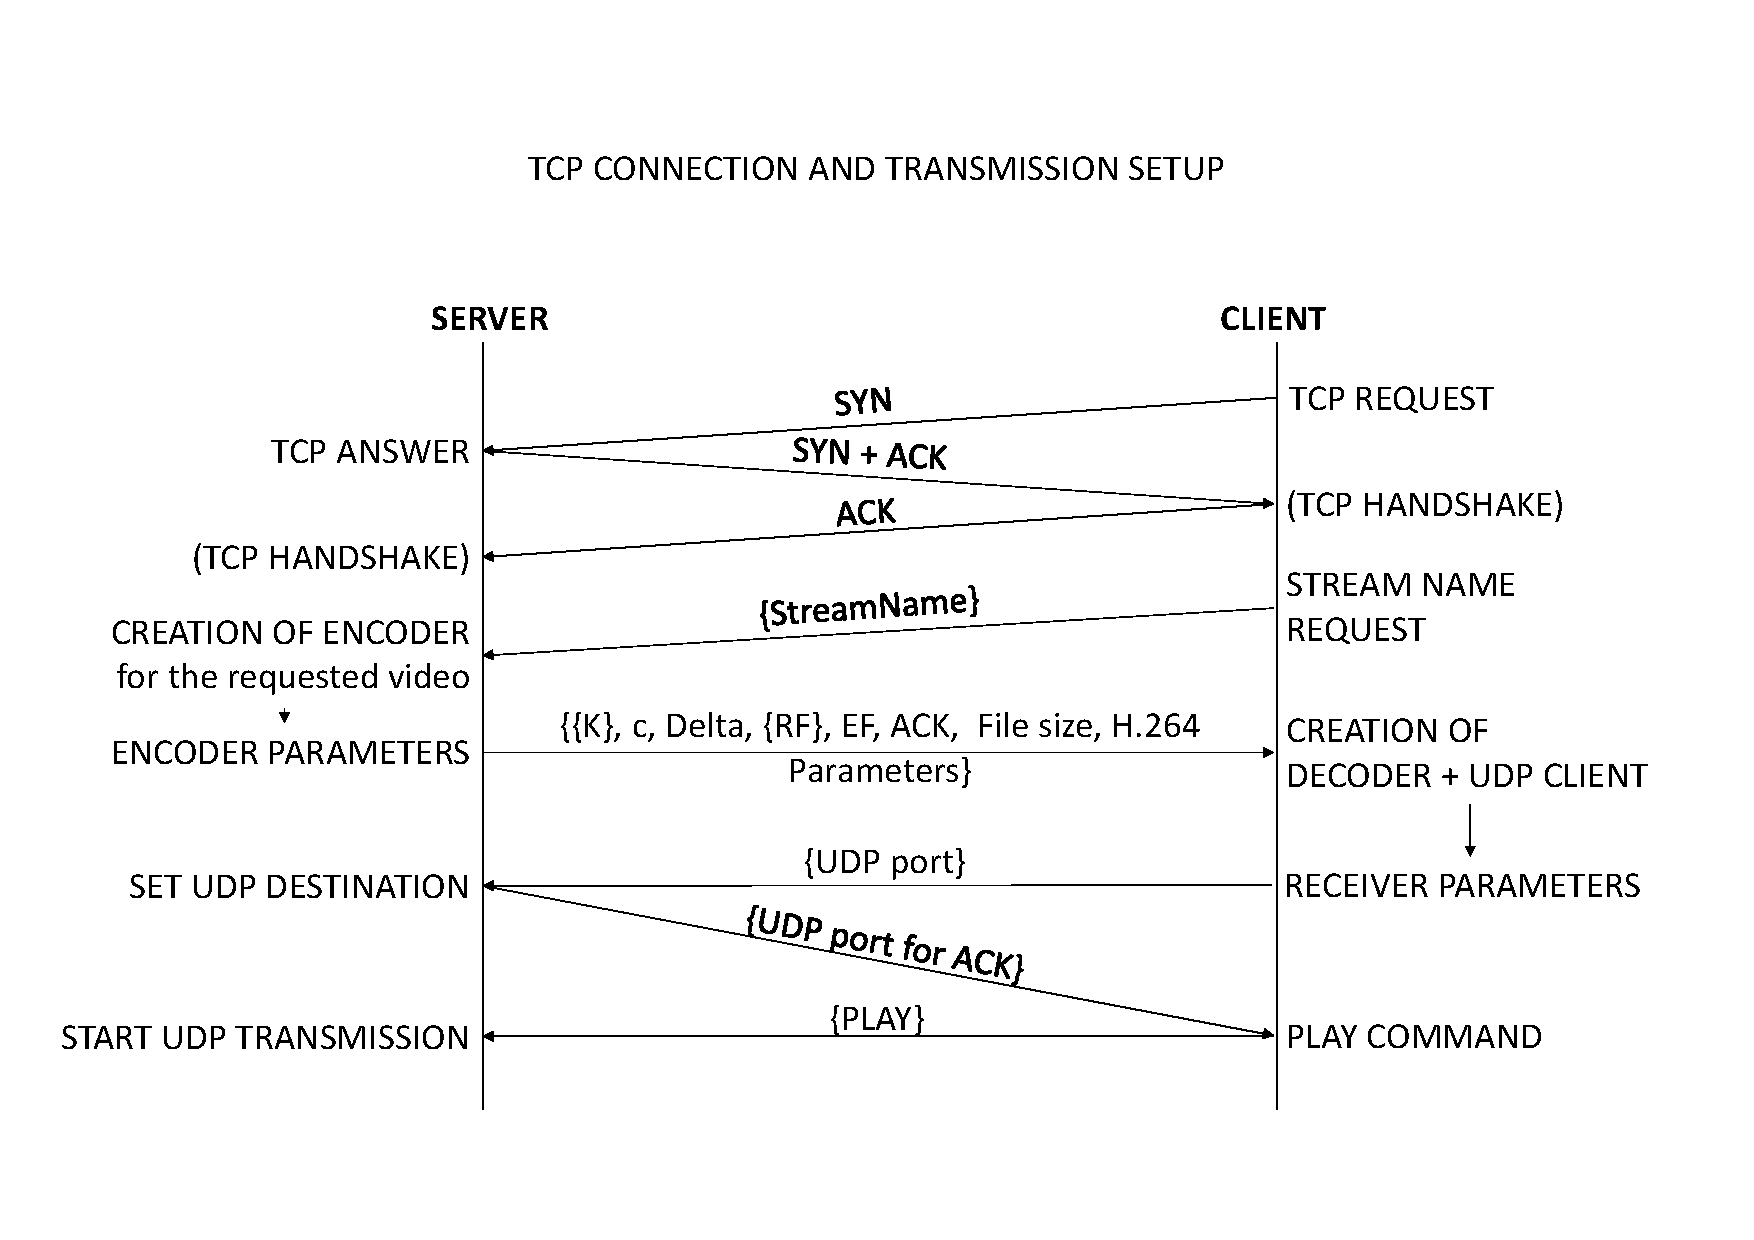
\includegraphics[clip, trim=0cm 1cm 0cm 1cm, width=1.00\textwidth]{TCP.pdf}
    \caption{TCP connection and tansmission setup}
    \label{fig:TCP}
\end{figure}
%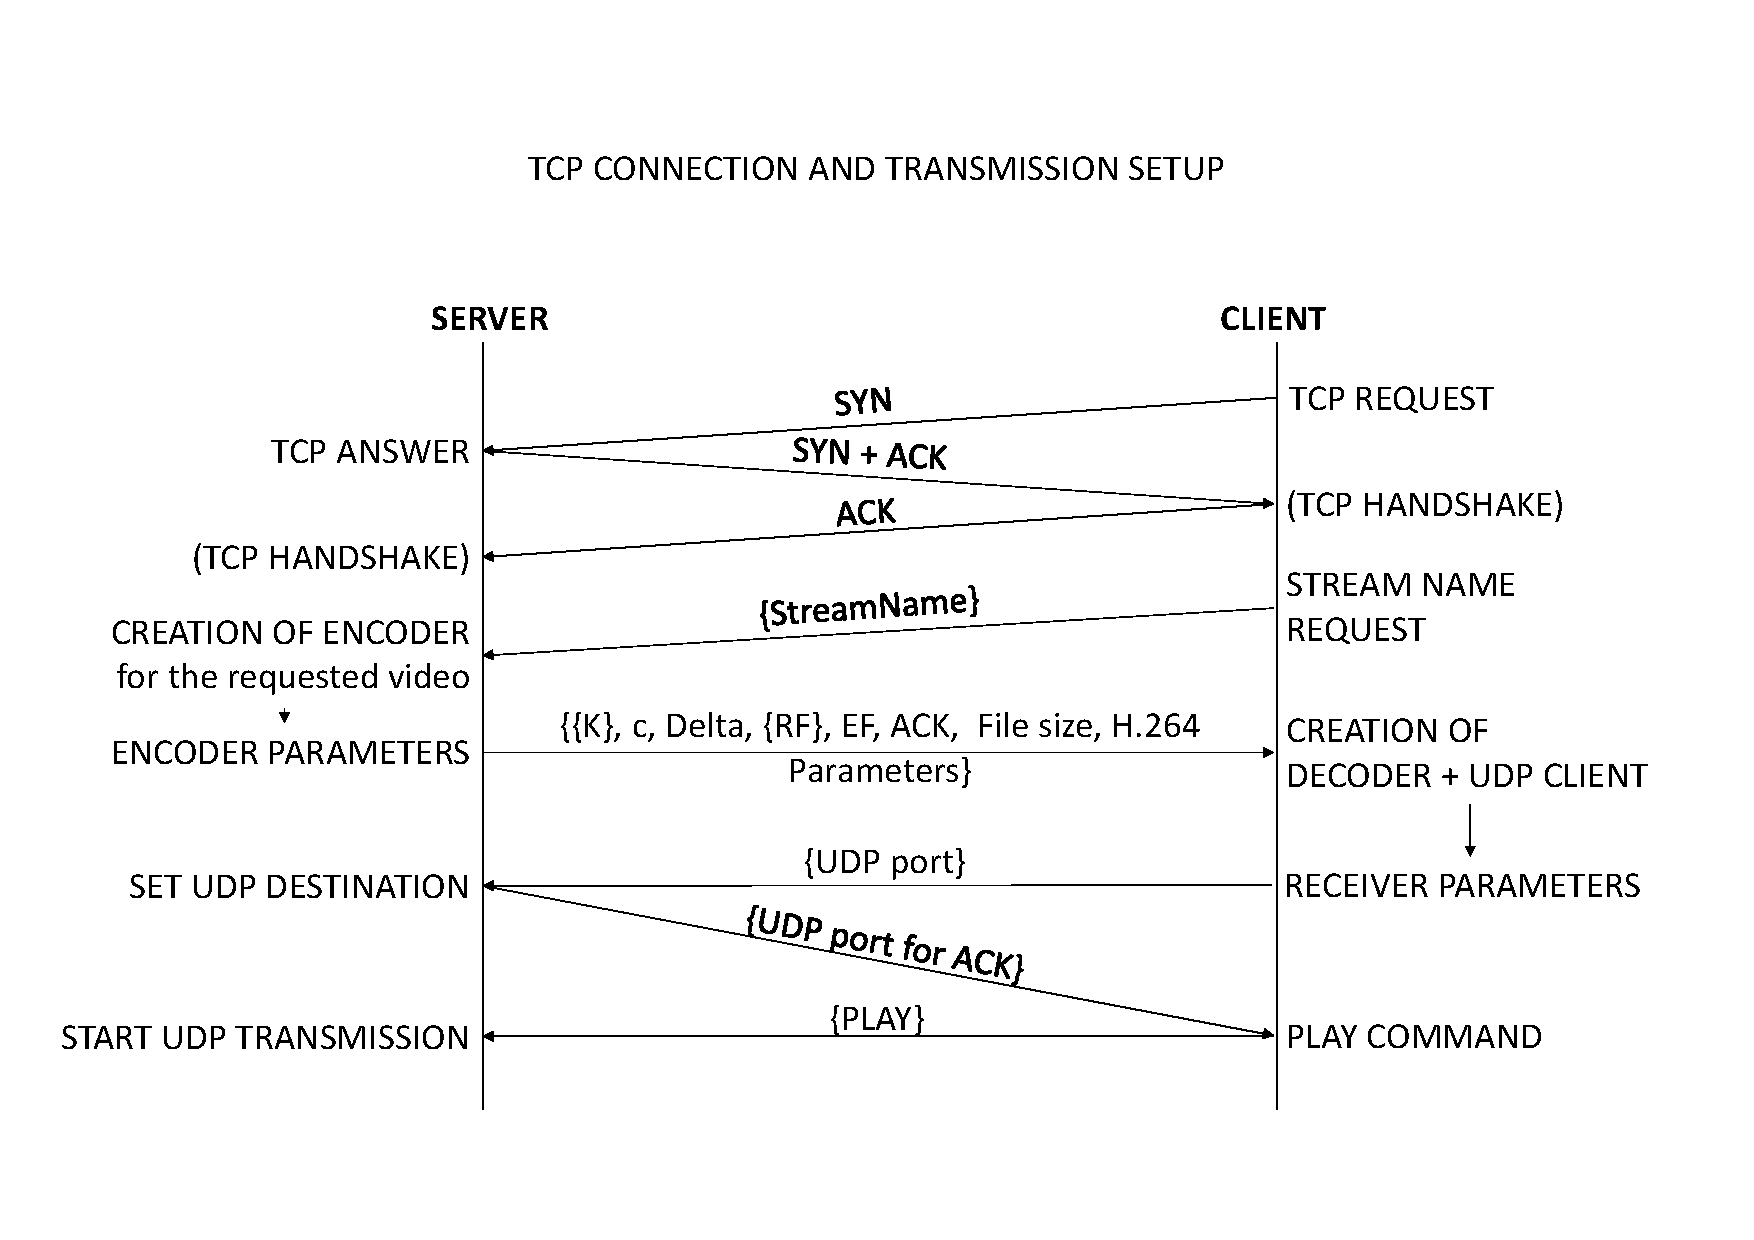
\includepdf{TCP.pdf}
\newpage
\subsection{Modelli matematici}
\subsubsection{Canale}
\label{sec:markov}
Il canale è rappresentato da una catena di Markov a 2 stati: buono (G) e cattivo (B).\\
Lo stato del sistema all'indice temporale $n$ (slot $n$) è indicato con $X(n)$, o $X_n$.\\
Sono stati effettuati test con due tipi di canale:
\begin{itemize}
\item Canale Markoviano, caratterizzato dalla seguente matrice di probabilità di transizione:\\
$$P=\begin{pmatrix}
P[X_n=G, X_{n+1}=G] & P[X_n=G, X_{n+1}=B]\\
P[X_n=B, X_{n+1}=G] & P[X_n=B, X_{n+1}=B]\\
\end{pmatrix} = \begin{pmatrix}
P_{GG} & P_{GB} \\
P_{BG} & P_{BB}
\end{pmatrix} =
\begin{pmatrix}
1-p & p \\
q & 1-q
\end{pmatrix}$$
Le probabilità stazionarie sono definite come
$$\bm{\pi} = \begin{pmatrix}
\pi_G\\\pi_B
\end{pmatrix} = \lim_{n \to\infty} \begin{pmatrix}
P[X(n)=G]\\
P[X(n)=B]
\end{pmatrix}$$
e possono essere ricavate dall'equazione
$$P^T\cdot \bm{\pi} = \bm{\pi} \Leftrightarrow \begin{pmatrix}
\pi_G\\
\pi_B
\end{pmatrix}=
\begin{pmatrix}
\frac{q}{p+q}\\
\frac{p}{p+q}
\end{pmatrix}$$
La probabilità stazionaria che il canale sia nello stato B è la probabilità d'errore media:
$$E[P_e] = \pi_B$$
Può essere definita la variabile aleatoria $\#_B$ che indica il numero di slot in cui il sistema resta nello stato B, la cui distribuzione di probabilità può essere scritta come:
$$P[\#_B=k]= \left(P_{BB}\right)^{k-1}P_{BG} = (1-q)^{k-1} q$$
Il valore atteso di $\#_B$ è l'inverso della probabilità di transizione da B a G:
$$E[\#_B] = \sum_{k=0}^{+\infty} k \cdot (1-q)^{k-1} q = q \cdot \frac{1}{(1-(1-q))^2} = \frac{1}{q}$$
I parametri impostati per il canale simulato sono stati il numero medio di slot B consecutivi, $E[\#_B]$, e la probabilità d'errore media $\pi_B$. In seguito sono state ricavate le seguenti quantità:
\begin{equation}
  \begin{cases}q = \frac{1}{\EnB}\\
\pi_G = 1- \pi_B\\
p = q\frac{\pi_B}{\pi_G}\end{cases}
  \label{eq:mcparams}
\end{equation}
Il numero medio di iterazioni necessarie a sbagliare N pacchetti è, in media,
$$E[\theta_{0N}] = \frac{\pi_G}{p} + \frac{N-1}{\pi_B}$$
Un altro tipo di canale markoviano testato è stato mantenendo fissa la quanità $\EnB$ e facendo variare la probabilità d'errore $\pi_B$.
\item Canale senza memoria, con packet error rate fisso $P_e$
\end{itemize}
Di seguito la rappresentazione Markoviana.
\begin{figure}[H]
    \centering
        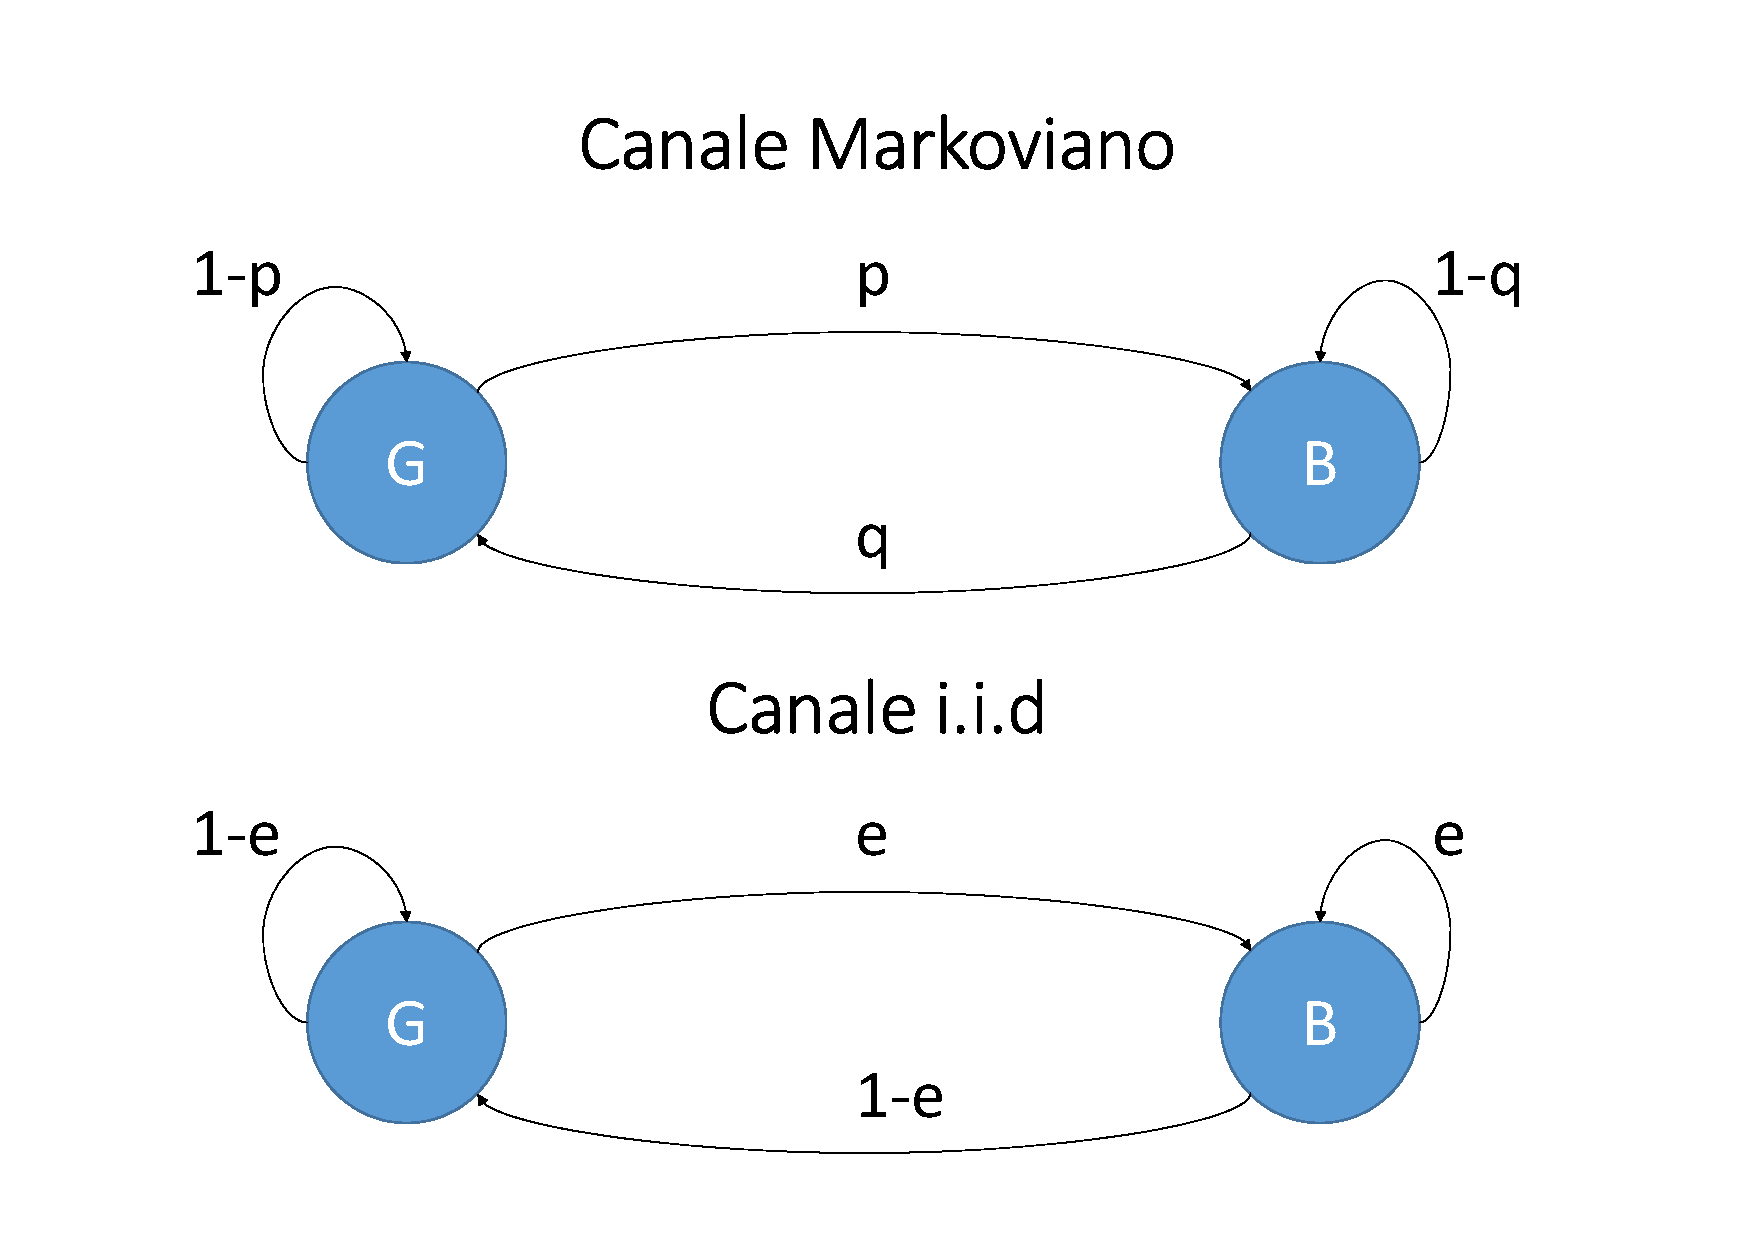
\includegraphics[clip, trim=0cm 1cm 0cm 1cm, width=0.5\textwidth]{Channel.pdf}
    \caption{Rappresentazione Markoviana dei due tipi di canale analizzati}
    \label{fig:Channel}
\end{figure}
\subsubsection{Codici a fontana}\label{FCsection}
I codici a fontana sono una classe di codici di correzione degli errori che aggiunge a un messaggio $\bm{x}\in\mathcal{A}^K$, di lunghezza $K$, una quantità di ridondanza potenzialmente infinita, aumentando la lunghezza del messaggio codificato $\bm{y}\in\mathcal{A}^N$, in modo tale che sia possibile recuperare il messaggio originale da un sottoinsieme di cardinalità leggermente maggiore di $K$ (e minore di $N$) del messaggio codificato.\\
%L'overhead introdotto dalla codifica è dato da $t = \frac{N-K}{K}$.\\
Fissando la lunghezza del messaggio codificato, $N$, per ogni messaggio originale di lunghezza $K<N$, è possibile schematizzare la codifica di canale lineare attraverso la seguente equazione
\begin{equation}
\bm{y} =
\begin{pmatrix}
y_1 \\y_2 \\y_3 \\\vdots \\y_N
\end{pmatrix} = \underbrace{\begin{pmatrix}
g_{11}	&g_{12}	&\cdots	&g_{1K}\\
g_{21}	&g_{22}	&\cdots	&g_{2K}\\
g_{31}	&g_{32}	&\cdots	&g_{3K}\\
\vdots &\ddots & \ddots &\vdots\\
g_{N1}	&g_{N2}	&\cdots	&g_{NK}
\end{pmatrix}}_{=G} \begin{pmatrix}
x_1 \\x_2 \\\vdots \\x_K
\end{pmatrix} = G \cdot \bm{x}
\end{equation}
dove $G$ è la matrice di codifica, $g_{ij}\in\{0,1\}$, $x_i\in\mathcal{X}$, $y_i\in\mathcal{Y}$.\\
La $i-$esima riga della matrice $G$ è casuale e il suo grado (la distanza di hamming dall'origine) segue una distribuzione di probabilità nota: la Robust Soliton Distribution.\\
La codifica dell'$i-$esimo pacchetto avviene attraverso l'operazione di \textit{OR esclusivo} tra i pacchetti di informazione indicati dalla $i-$esima riga di $G$.\\
Se $G$ è invertibile, è possibile recuperare il vettore $\bm{x}$ da $\bm{y}$ attraverso la risoluzione di un sistema lineare.\\
I codici a fontana non prevedono la risoluzione di un sistema lineare per la decodifica, bensì un algoritmo di \textit{message passing}: con riferimento alla figura (\ref{fig:FC})
\begin{itemize}
        \item SE esiste un simbolo codificato $e_n$ con un solo arco entrante (come $e_4$)\begin{itemize}
                \item	Decodifica il simbolo di informazione corrispondente $i_k=e_n$ ($i_5$ in questo caso)
                \item	Rimpiazza tutti i simboli codificati $e_{n'}$ aventi un arco entrante da $i_k$ con $e_{n'}^{\text{new}} = e_{n'} \textit{ XOR } i_k$
                \item   Rimuove gli archi da $i_k$
                \item   SE ci sono altri simboli di informazione da decodificare \begin{itemize}
                        \item Torna all'inizio
                \end{itemize}
                \item ALTRIMENTI\begin{itemize}
                        \item Decodifica riuscita
                \end{itemize}
        \end{itemize}

        \item ALTRIMENTI Decodifica fallita
\end{itemize}
\begin{figure}[H]
    \centering
        \makebox[\textwidth][c]{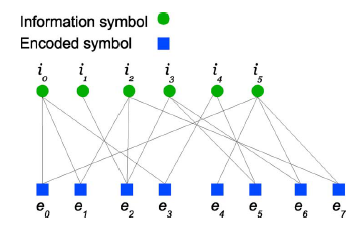
\includegraphics[width=6cm]{fc.png}}
    \caption{Schema: \textit{message passing}}
    \label{fig:FC}
\end{figure}
\newpage
\subsubsection{H.264}
Più nel dettaglio, il flusso video codificato è organizzato in unità NAL (Network Abstraction Layer) che possono essere di 2 tipi: VCL NAL Packets (Video Coding Layer) e non-VCL NAL packets. I pacchetti non-VCL possono contenere il set di parametri da usare per decodificare (informazioni necessarie per la decodifica, quindi ad alta priorità), oppure delle informazioni supplementari per migliorare la decodifica (SEI, Supplemental Enhancement Information). Il bitstream NAL è composto da una serie di sequenze video più corte (GOP, Group Of Pictures) decodificabili indipendentemente dal resto del flusso: ogni GOP comincia con tutte le informazioni necessarie alla decodifica, in modo che essa possa avvenire anche senza aver decodificato nessun segmento precedente.\\
Un tipo di applicazione che si presta particolarmente all'utilizzo di UEP \cite{uep} è lo streaming di un video codificato attraverso SVC, infatti tale protocollo rende possibile la decodifica di un flusso video da flussi parziali, chiamati \textit{layer}, con risoluzione spaziale o temporale minore, o con fedeltà ridotta. I layer sono ordinati dal più importante (layer 0, a bassa qualità) al meno importante (layer \textit{n}, che permette di raggiungere alta qualità).\\
La presenza di informazioni più rilevanti di altre (come i parametri per la decodifica e i layer inferiori, in particolare i frame intra-coded) giustifica l'uso di UEP: i flussi con priorità minore aggiungono qualità al video decodificato, ma non sono indispensabili per la decodifica, quindi possono essere protetti con meno ridondanza.
\subsubsection{UEP}\label{UEPsection}
La protezione non uniforme di un messaggio prevede la divisione dello stesso in $p$ parti di diversa importanza.\\
Ogni parte viene ripetuta un numero $RF_i$ di volte, con $i\in\{1,\cdots,p\}$, in base alla sua importanza.\\
Il risultato della giustapposizione delle parti ripetute viene a sua volta ripetuto un numero $EF$ di volte.\\
Il messaggio che si ottiene da tali giustapposizioni è mappato nelle parti originali del messaggio originale e viene inviato al codificatore a fontana. Di seguito uno schema rappresentativo con $p=2$, $RF_1 = 2$,$RF_2=1$, $EF=2$.
\begin{figure}[H]
    \centering
        \makebox[\textwidth][c]{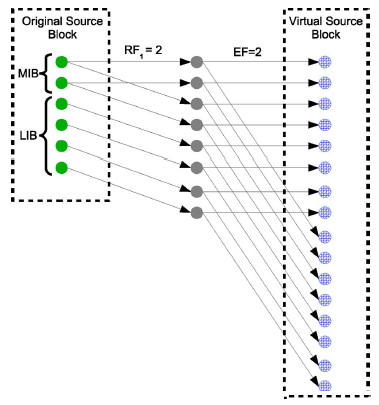
\includegraphics[width=8cm]{uep.png}}
    \caption{Schema della protezione non uniforme}
    \label{fig:UEP}
\end{figure}
\newpage
\subsection{Complicazioni trovate} % Max 5 lines

\section{Risultati} % Min 7 pages
L'algoritmo per la protezione non uniforme esposto nel
paragrafo~\ref{UEPsection} è stato testato nei due casi di canale
senza memoria e di canale Markoviano per determinare la packet error
rate ottenibile in queste due condizioni.

Sono stati inoltre misurati i tempi necessari alla codifica e
decodifica dei pacchetti in funzione dell'overhead desiderato.

Purtroppo l'esecuzione dell'intera implementazione dello schema di
figura~\ref{fig:UDP} richiede un tempo tale da rendere difficoltosa la
costruzione di grafici che siano precisi per PER basse.
%
I risultati dei paragrafi seguenti sono, quindi, stati ottenuti
utilizzando solamente l'implementazione del message passing, senza
trasmettere realmente dei pacchetti.

\subsection{Packet error rate su un canale senza memoria}
In questo caso è stata misurata la packet error rate a livello di
applicazione ottenuta variando l'overhead e considerando diversi
valori per la packet error rate del canale.
%
Facendo riferimento alla figura~\ref{fig:UDP}, la PER di livello
applicazione è la frazione di pacchetti forniti all'UEP encoder che
raggiungono l'uscita dell'UEP decoder, che corrisponde alla frazione
di pacchetti decodificati dal message passing.
%
L'overhead è definito, in modo analogo a \cite{uep}, come $t =
\frac{N-K}{K}$, dove $N$ è il numero di pacchetti codificati prodotti
per ogni blocco e $K$ è la dimensione del blocco.
%
Il canale iid è simulato scartando con probabilità $e$ ognuno degli
$N$ pacchetti codificati.

I valori per i parametri sono stati scelti come in \cite{uepother},
una versione precedente di \cite{uep}, perché permettono di
evidenziare meglio il diverso comportamento della PER relativa ai
pacchetti importanti rispetto al resto del blocco.

Sono stati usati blocchi contenenti $K_0 = 100$ pacchetti importanti e
$K_1 = 1900$ pacchetti non importanti, il blocco virtuale è stato
costruito ripetendo $RF_0 = 5$ volte il primo sotto-blocco, $RF_1 = 1$
volte il secondo ed espandendo la sequenza di pacchetti così ottenuta
di un fattore $EF = 2$. La lunghezza del blocco virtuale è quindi pari
a $EF \cdot \left( RF_0 \cdot K_0 + RF_1 \cdot K_1 \right) = 4800$
pacchetti.
%
L'overhead è stato fatto variare nell'intervallo $[0, 0.8]$, a cui
corrisponde un numero di pacchetti inviati $N \in [2000, 3600]$ per
ogni blocco di $K=K_0+K_1$ pacchetti.
%
La probabilità di errore del canale è stata impostata ai valori $e \in
\left\{10^{-2}, 10^{-1}, 3 \cdot 10^{-1} \right\}$, oltre al caso
senza errori con $e=0$.

Nelle figure~\ref{fig:zero_oh} e~\ref{fig:iid_oh} sono mostrati i
risultati della simulazione di 10000 blocchi.
%
\begin{figure}[htb]
  \centering
  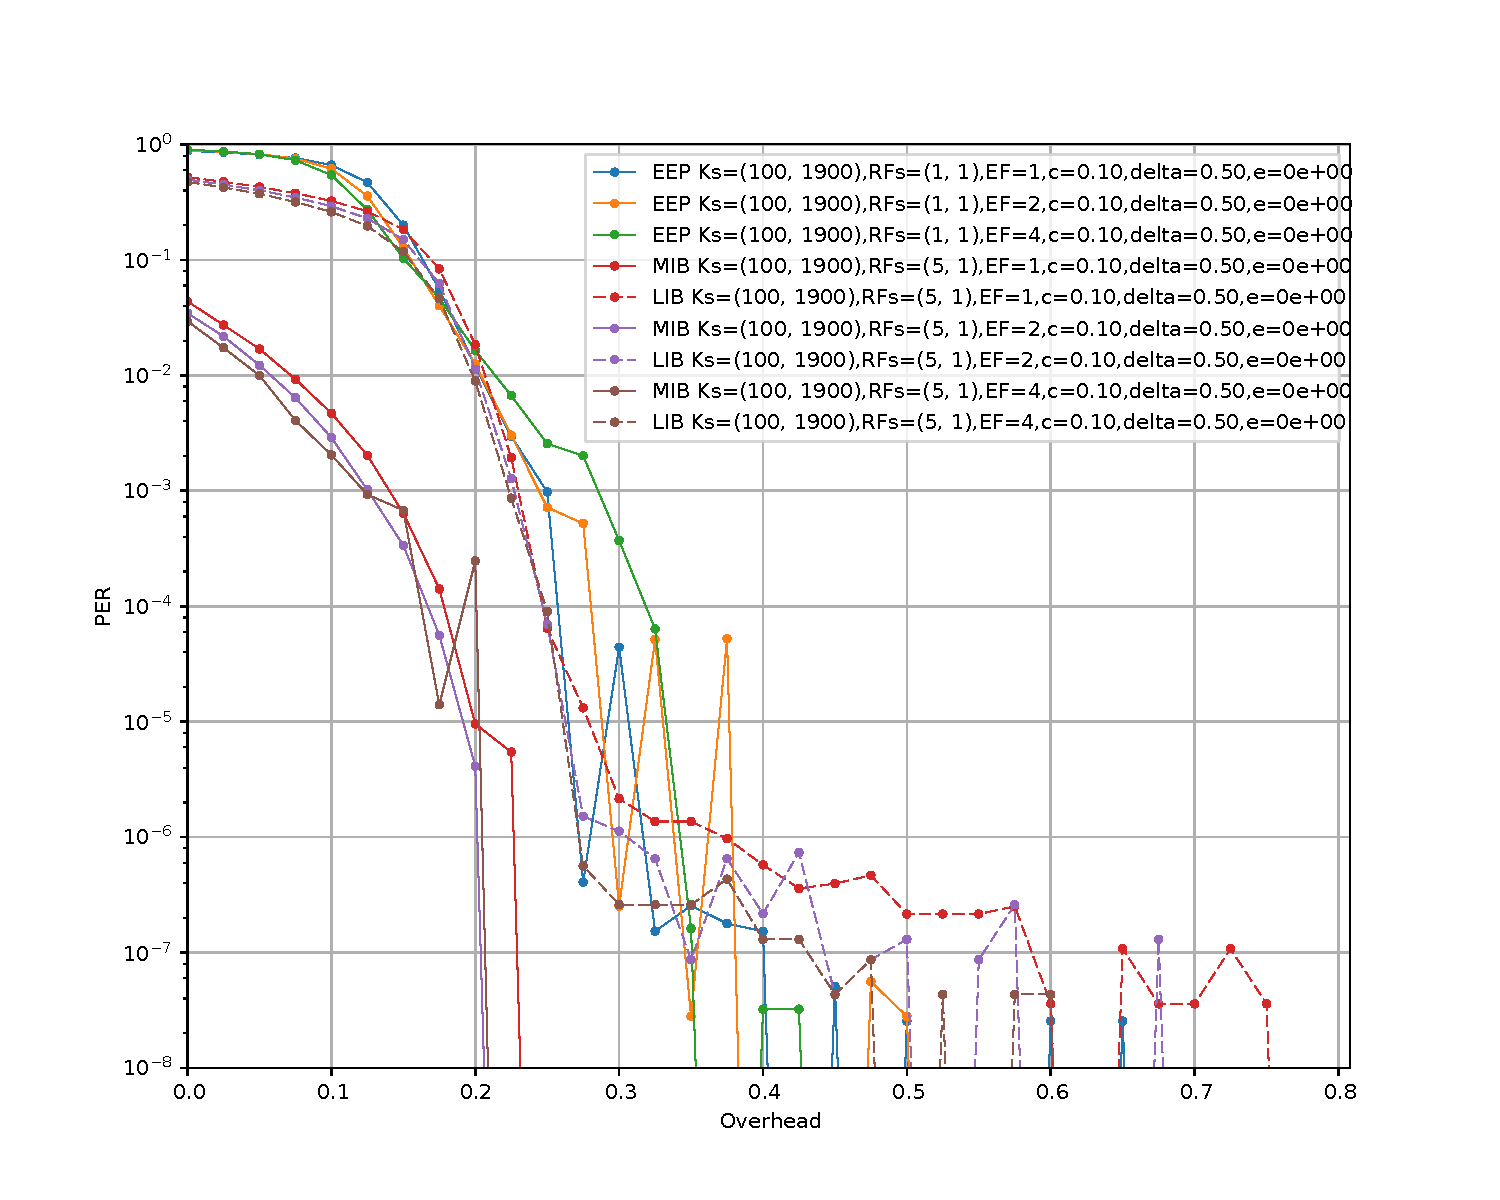
\includegraphics[width=0.8\textwidth]{plot_ber_zero_oh}
  \caption{Packet error rate al variare dell'overhead su un canale
    senza errori.}
  \label{fig:zero_oh}
\end{figure}
% Plot notes:
% better EEP EF=1 for 0.2 - 0.4 -> [8:17] or more
% Remove EEP EF>1 because worse PER after oh=0.18
% UEP EF = 4: better points in [4:17]
% UEP EF = 2: better points in [11:17]
%
\begin{figure}[htb]
  \centering
  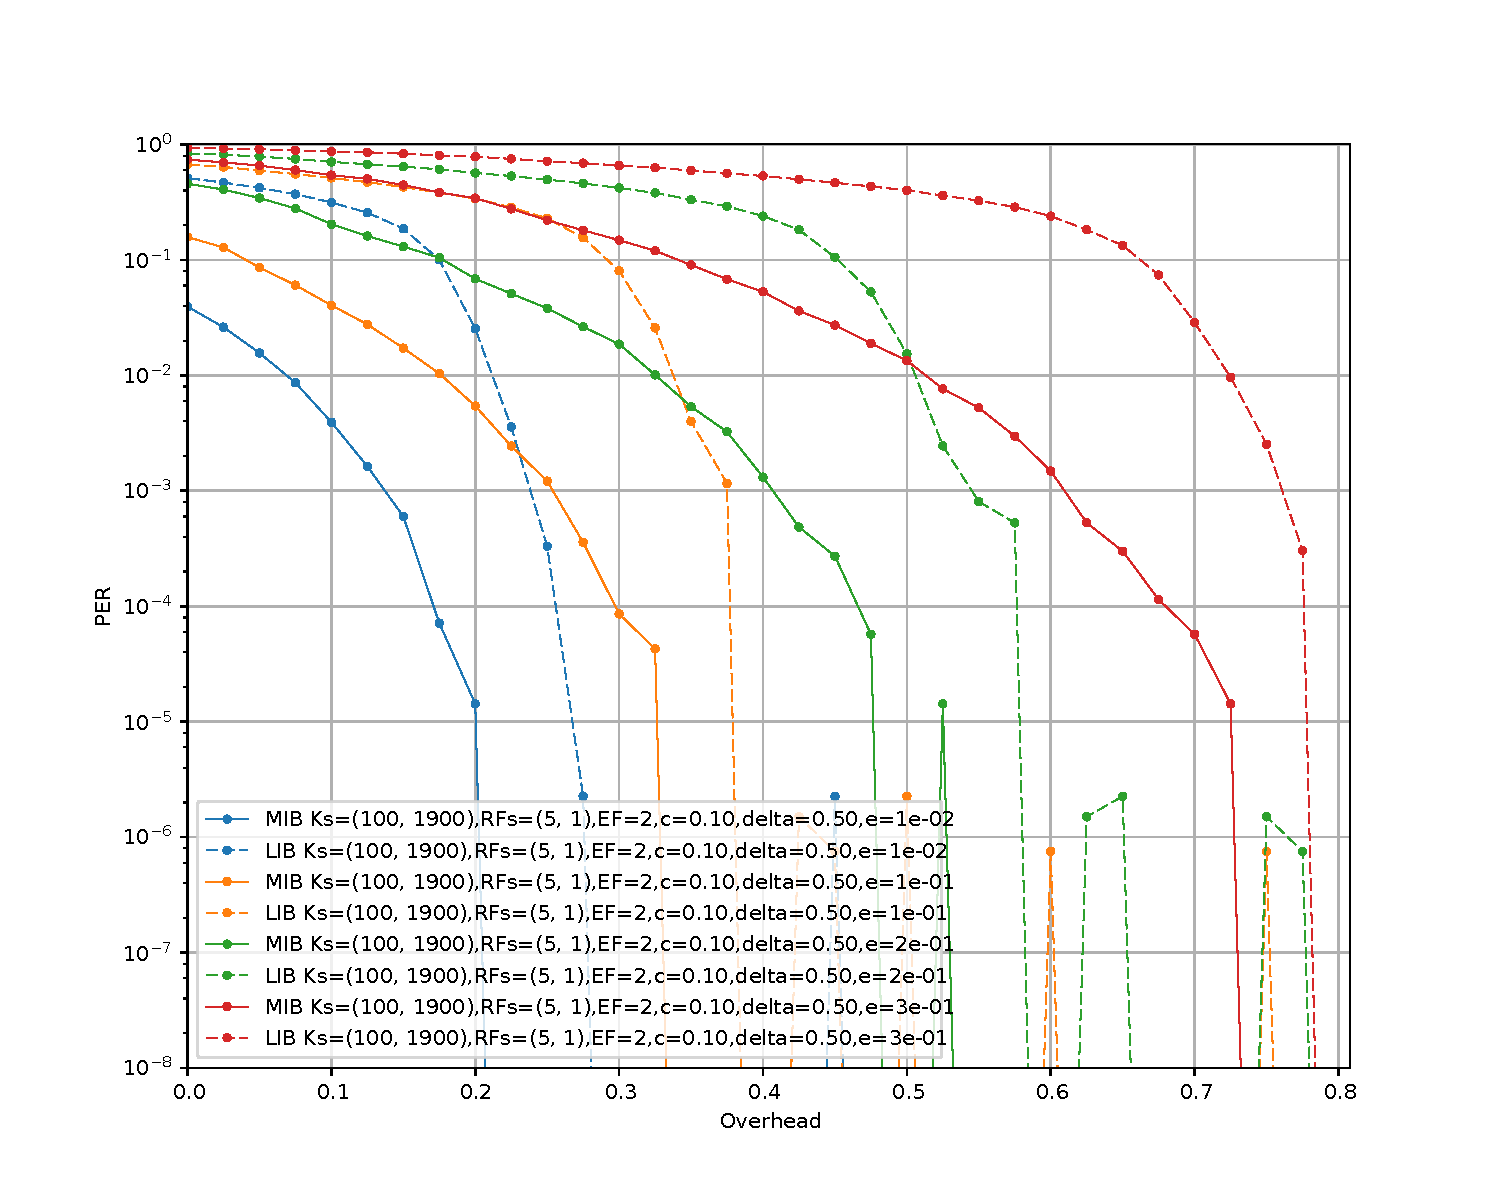
\includegraphics[width=0.8\textwidth]{plot_ber_iid}
  \caption{Packet error rate al variare dell'overhead su un canale
    iid.}
  \label{fig:iid_oh}
\end{figure}
% Plot notes:
% more points everywhere

% Markov plot notes:
% Error-free:
% EEP is good, more between 2000-4000 -> [8:12]
% UEP RF=5 more points everywhere for the LIB +
%   [4:9]
%
% BR5:
%

Nel caso senza errori (figura~\ref{fig:zero_oh}) si può vedere come la
scelta dei vettori di codifica che predilige i pacchetti importanti
fornisca un miglioramento nella PER relativa a questi ultimi, rispetto
al caso EEP.
%
D'altro canto vediamo come la PER relativa ai pacchetti meno
importanti, anche se inizialmente è migliore del caso EEP, al crescere
dell'overhead decresce più lentamente e rimane sopra a $10^{-8}$ per
tutto l'intervallo considerato.
%
Il fattore di espansione $EF$ non fornisce miglioramenti significativi
della PER del MIB, mentre permette di diminuire la PER del LIB per gli
overhead più alti. Con $EF > 2$, tuttavia, questo effetto tende a
diventare sempre più piccolo.

Dal grafico delle PER per il caso in cui il canale perde pacchetti in
modo iid (figura~\ref{fig:iid_oh}) è possible vedere che le curve
seguono lo stesso andamento del caso precedente. Sono semplicemente
traslate al variare della PER del canale di una lunghezza di circa
$1.6$ volte il valore della PER.
%
Infatti, nel caso $e = 10^{-2}$ l'algoritmo testato ha delle
prestazioni molto vicine a quelle ottenibili sul canale senza errori,
mentre nei casi con PER $e = 10^{-1}$ ed $e = 3\cdot 10^{-1}$ le curve
siano traslate, rispettivamente, circa di $0.16$ e $0.48$ rispetto al
caso senza errori.

\subsection{Packet error rate su un canale Markoviano}
Nel caso del canale Markoviano, descritto nel
paragrafo~\ref{sec:markov}, sono state eseguite simulazioni per
valutare la packet error rate considerando canali con diverse
lunghezze medie $E[\#_B]$ di una sequenza di slot cattivi consecutivi
e variando la dimensione del blocco $K$.
%
In modo analogo al paragrafo precedente, il canale è stato simulato
facendo una transizione di stato prima di ogni nuovo pacchetto e
scartando quest'ultimo in caso lo stato sia ``cattivo''. Lo stato
iniziale è stato in modo iid per ogni blocco di pacchetti, secondo le
probabilità stazionarie $\pi_G$ e $\pi_B$.

La frazione di pacchetti importanti presente in ogni blocco è stata
mantenuta al 5\%, come per il caso iid, e anche per gli altri
parametri sono stati usati valori simili: $RF_0 = 5$, $RF_1 = 1$,
$EF=2$, $c=0.1$, $\delta=0.5$. Il numero di pacchetti trasmessi $N$ è
stato fissato per avere un overhead del 30\%.

Nella figura~\ref{fig:markov_zero} possiamo vedere il caso del canale
senza errori al variare di $K$.
%
\begin{figure}[htb]
  \centering
  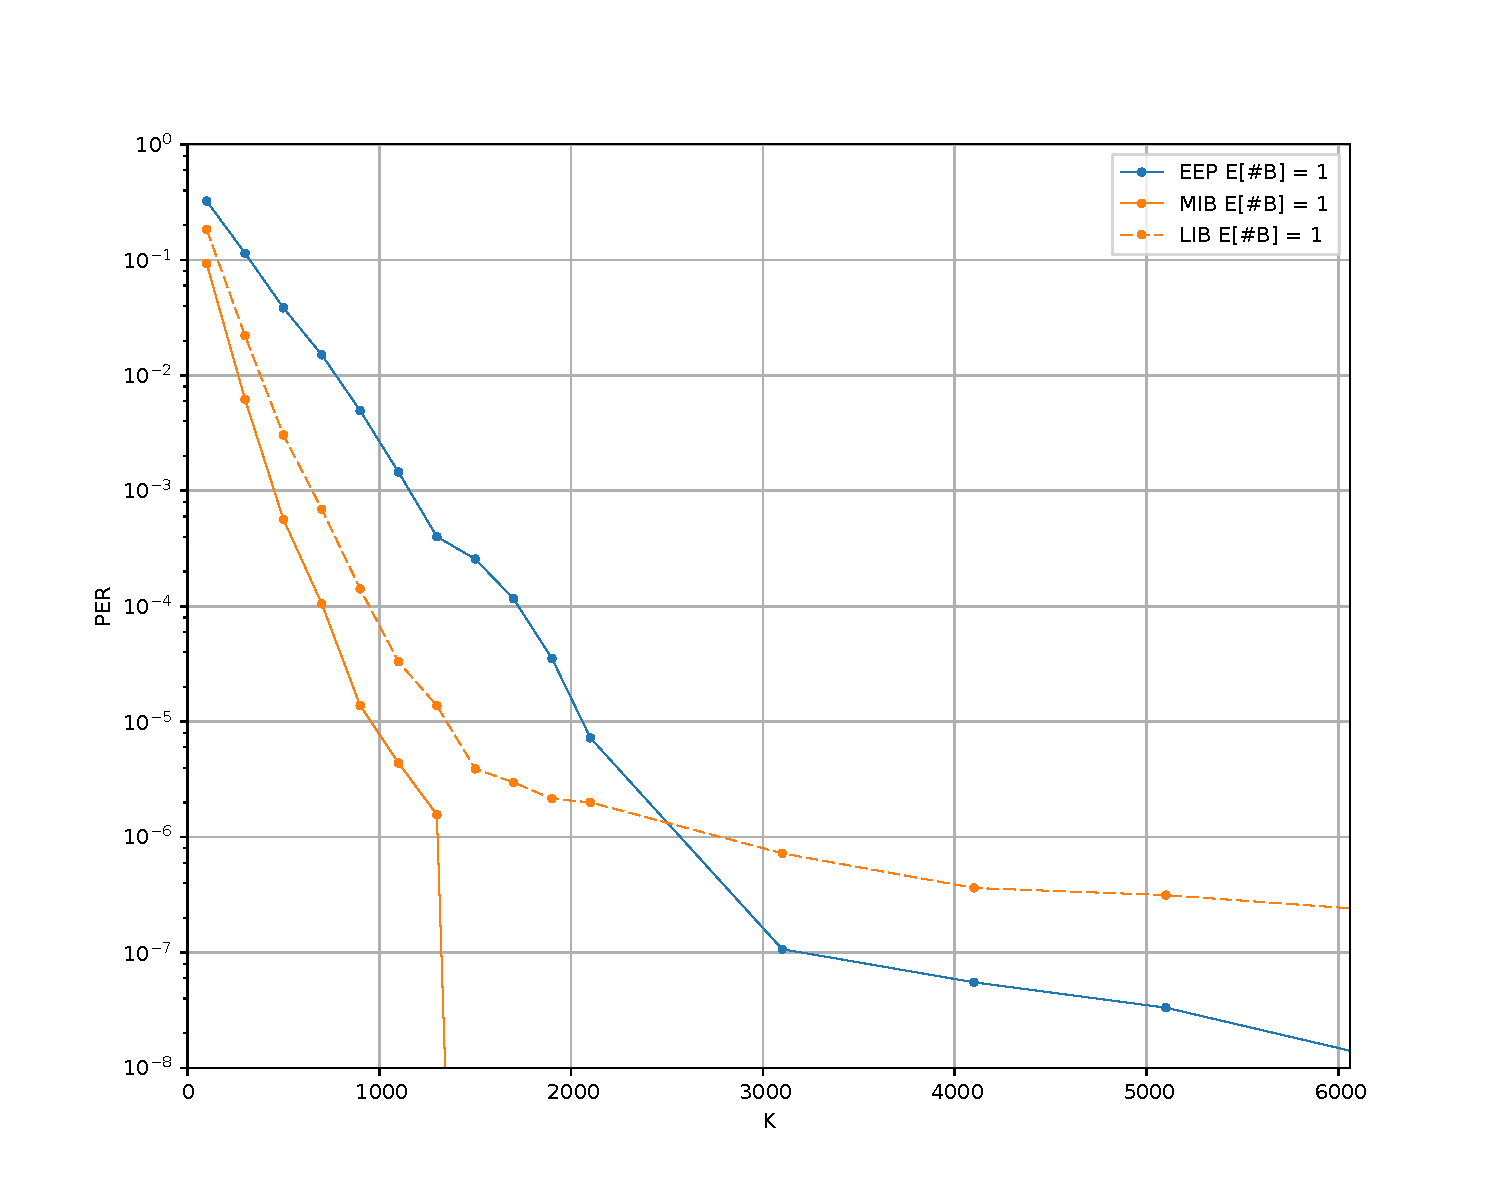
\includegraphics[width=0.8\textwidth]{plot_markov_zero}
  \caption{Packet error rate a livello applicazione ottenuta al
    variare della dimensione del blocco sul canale error-free.}
  \label{fig:markov_zero}
\end{figure}
%
Vediamo che anche nel caso del canale perfetto la probabiltà di errore
è molto alta in corrisponenza di blocchi piccoli e come, nel caso sia
applicata la UEP, sia possibile ottenere PER basse per il MIB molto
prima che nel caso EEP.

Se, invece, consideriamo sei diversi canali Markoviano fissando $\EnB
\in \{5,10,50\}$ e provando due diversi valori per la probabilità
media di errore $\pi_B \in \{0.01, 0.1\}$, possiamo vedere come gli
errori correlati influiscano sulla PER.
%
\begin{figure}[htb]
  \centering
  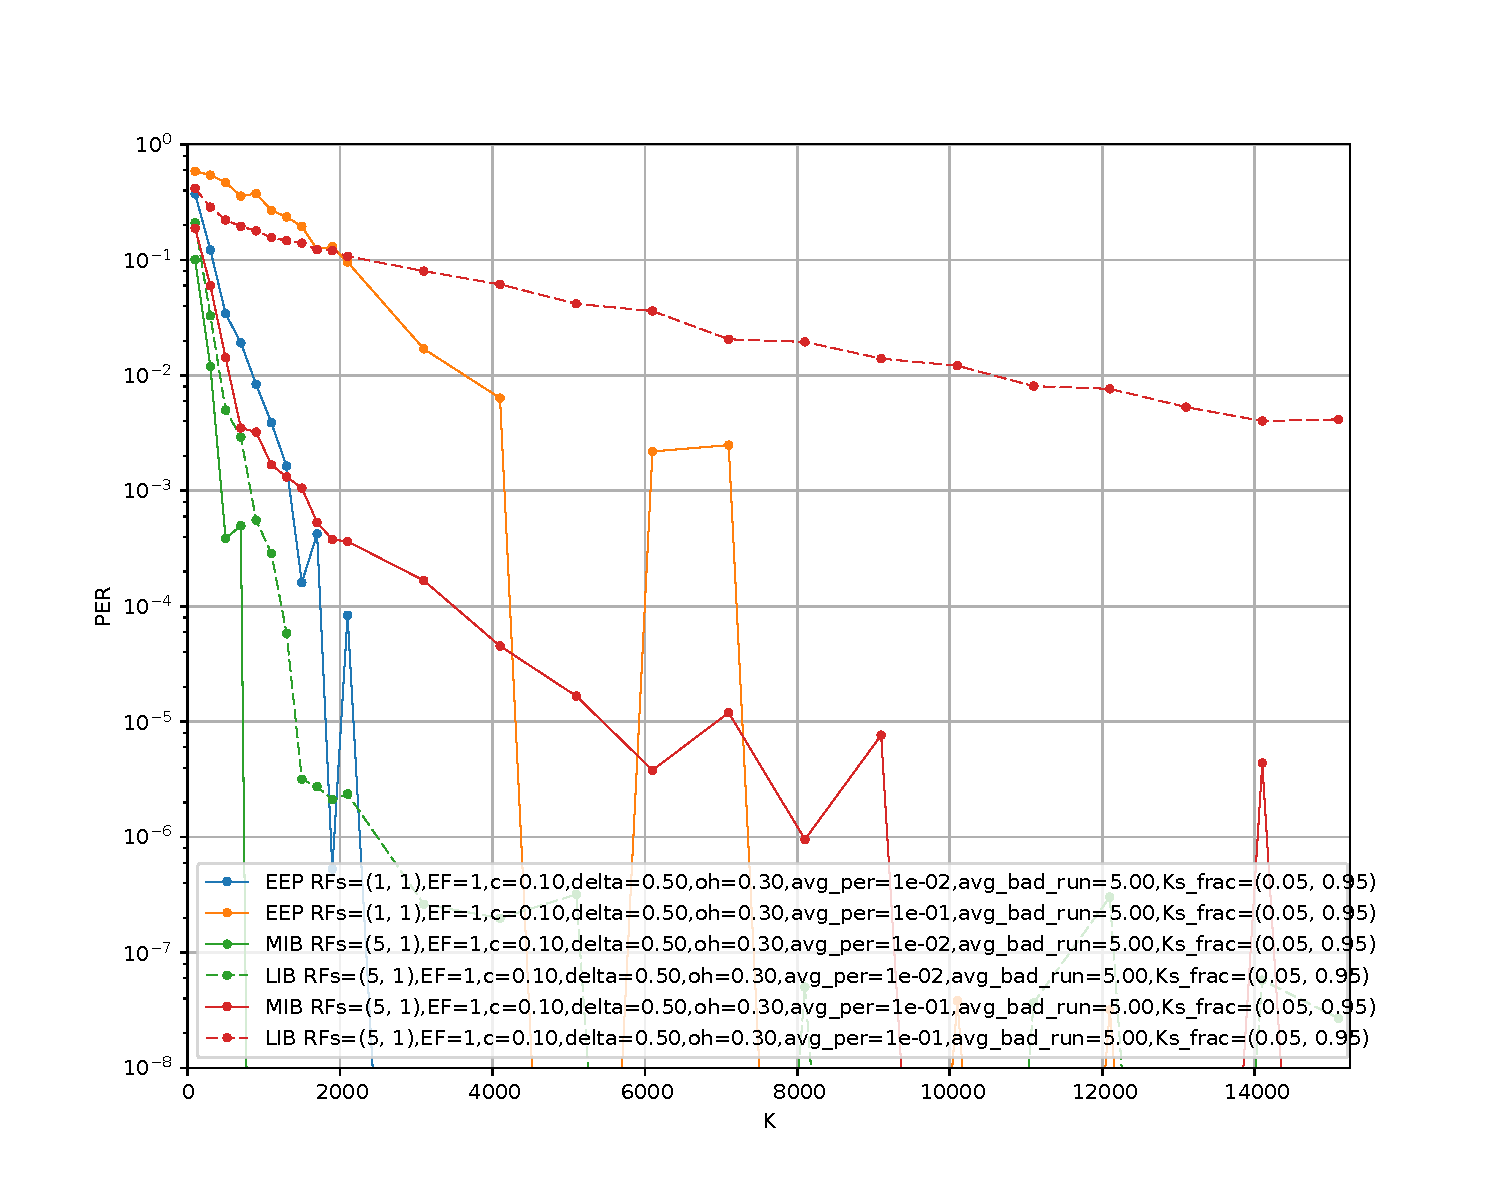
\includegraphics[width=0.8\textwidth]{plot_markov_br5}
  \caption{Packet error rate a livello applicazione ottenuta al
    variare della dimensione del blocco su due canali Markoviani con
    $\EnB = 5$ e $\pi_B \in \{0.01, 0.1\}$.}
  \label{fig:markov_br5}
\end{figure}
%
Se il canale offre una packet error rate media di $0.01$, possiamo
notare come il peggioramento delle prestazioni rispetto ai casi
error-free e iid (figura~\ref{fig:iid_oh}) non sia drastico: la PER
EEP scende a $10^{-8}$ in corrispondenza di $K \approx 2500, 4000,
5000$, rispettivamnte, per le tre lunghezze medie del burst; inoltre
in tutti e tre i casi il MIB ottiene un tasso di errore più basso del
caso EEP e peggiora altrettanto lentamente. Il LIB risente della
correlazione tra errori nello stesso modo: le curve scendono più tardi
a valori comparabili al caso error-free, ma la dimensione di blocco
necessaria non è molto più alta.

Per il caso con $\pi_B = 0.1$, invece, vediamo come la discesa della
PER sia molto più lenta. Per $K = 2000$ possiamo confrontare il
grafico con il caso iid e vedere come il peggioramento sia visibile ma
non di grande entità. Rispetto al caso con $\pi_B = 0.01$, tuttavia,
le PER del case UEP scendono molto lentamente: il LIB non riesce a
scendere sotto $10^{-3}$ nell'intervallo di $K$ considerato anche per
il burst più corto, e il MIB richiede blocchi molto più grandi per
scendere sotto $10^{-8}$. In questo caso le prestazioni della codifica
EEP, anche se inizialmente sono peggiori del LIB, scendono più
velocemente del MIB e permettono di ottenere una PER sotto $10^{-8}$
con blocchi più corti di quelli richiesti per il MIB.

Da tutto ciò possiamo vedere come, nel caso di errori correlati,
l'effetto della protezione non uniforme sia tanto più forte quanto
mggiore è la dimensione $K$ del blocco.
%% Il contrario, invece, accade nel caso error-free dove, al crescere
%% della dimensione del blocco, le probabilità di errore su MIB e LIB
%% tendono ad avvicinarsi \cite{uep}.

Si vede anche come la codifica riesca a correggere bene i burst di
errori quando la probabilità media di errore del canale non è molto
alta, infatti la PER raggiunge velocemente valori simili al caso IID e
offre una protezione dagli errori per il MIB migliore del caso EEP.
%
Se la PER del canale è alta rispetto all'overhead introdotto dalla
codifica, invece, le prestazioni sono drasticamente peggiori ed è
necessaria una dimensione di blocco molto alta per ottenere PER basse
sul MIB. In questo caso la codifica EEP diventa preferibile dopo una
certa dimensione del blocco.

\subsection{Tempi di codifica e decodifica}
Per verificare quanto tempo è necessario alla codifica e alla
decodifica di un blocco di pacchetti al variare dei parametri è stata
simulata la trasmissione di 500 blocchi al variare dell'overhead,
utilizzando lo stesso procedimento dei paragrafi precendenti.

Sono stati simulati sia il caso di equal error protection che quello
di unequal error protection, usando diversi valori per il fattore di
espansione $EF \in \{ 1,2,4 \}$. Gli altri parametri sono gli stessi
dei paragrafi precedenti: $K = 2000$, $K_0 = K \cdot 0.05$, $c=0.1$,
$\delta=0.5$ e per il caso UEP $RF_0 = 5$.

In figura~\ref{fig:encdec} sono mostrati i tempi medi di codifica e di
decodifica ottenuti eseguendo le simulazioni su una CPU Intel Xeon
E5450 con 16 GB di RAM.
%
\begin{figure}[htb]
  \centering
  \begin{subfigure}{0.5\textwidth}
    \centering
    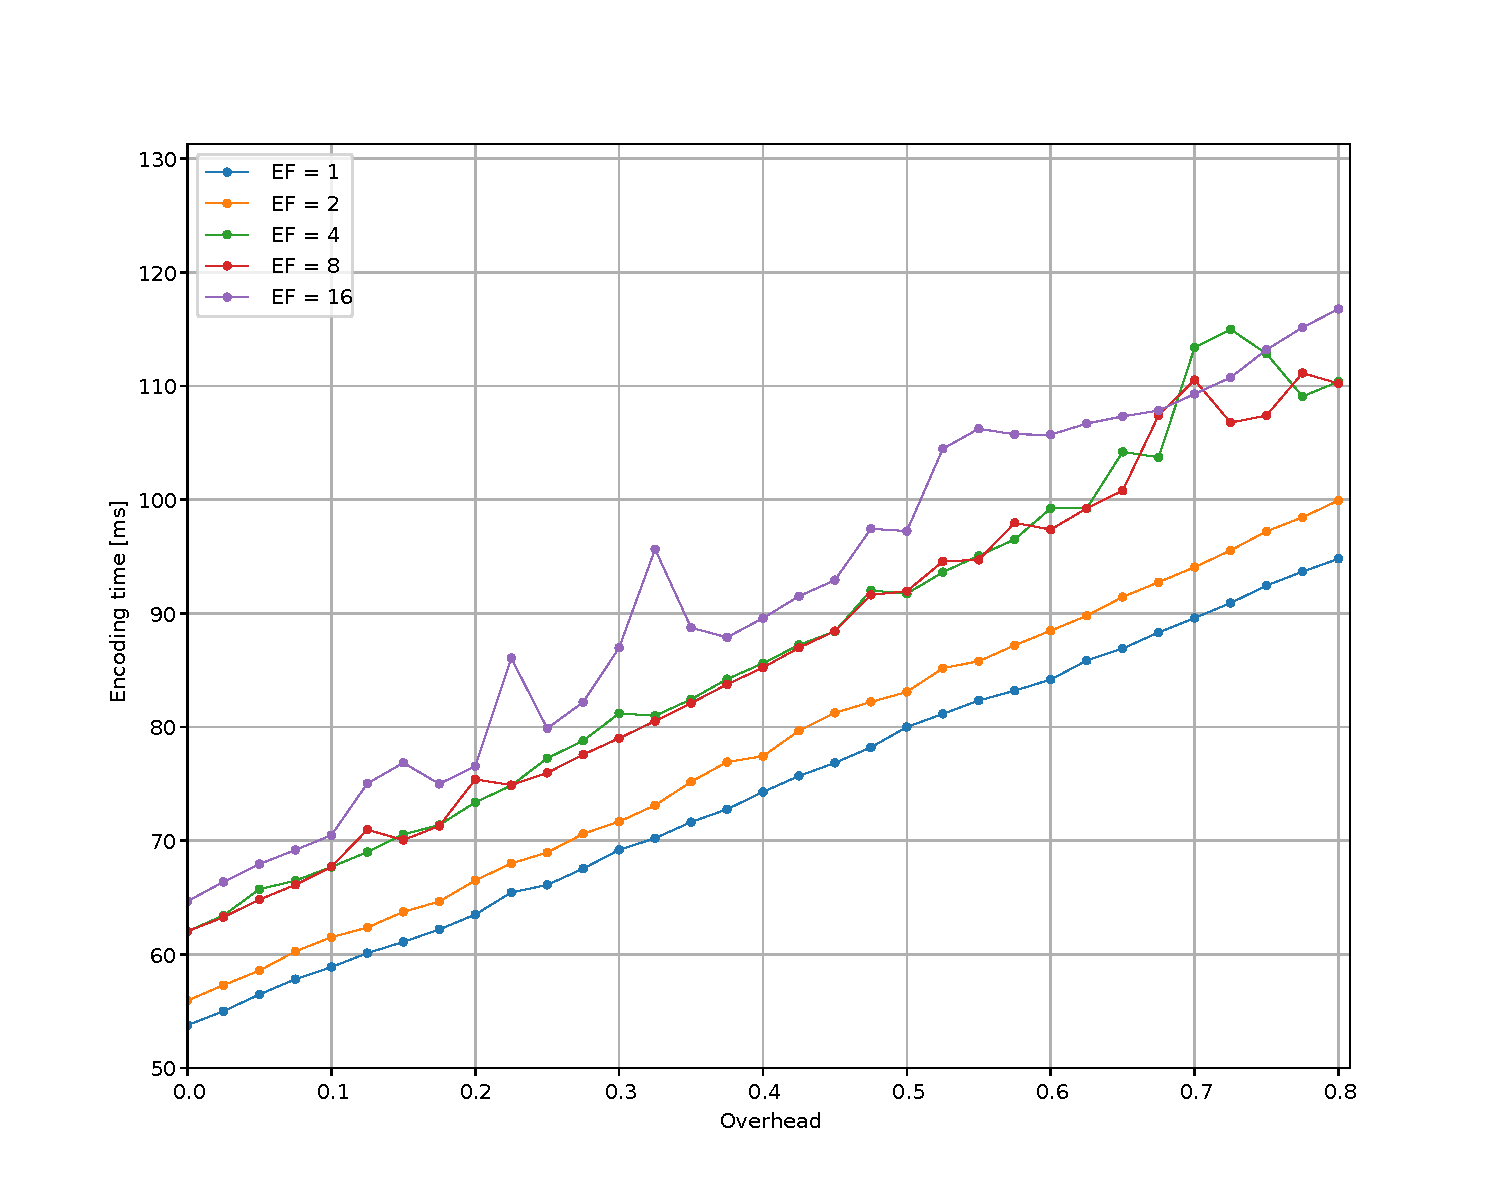
\includegraphics[width=\textwidth]{plot_enc_time_eep}
    \caption{Codifica EEP}
    \label{fig:enctime_eep}
  \end{subfigure}%
  \begin{subfigure}{0.5\textwidth}
    \centering
    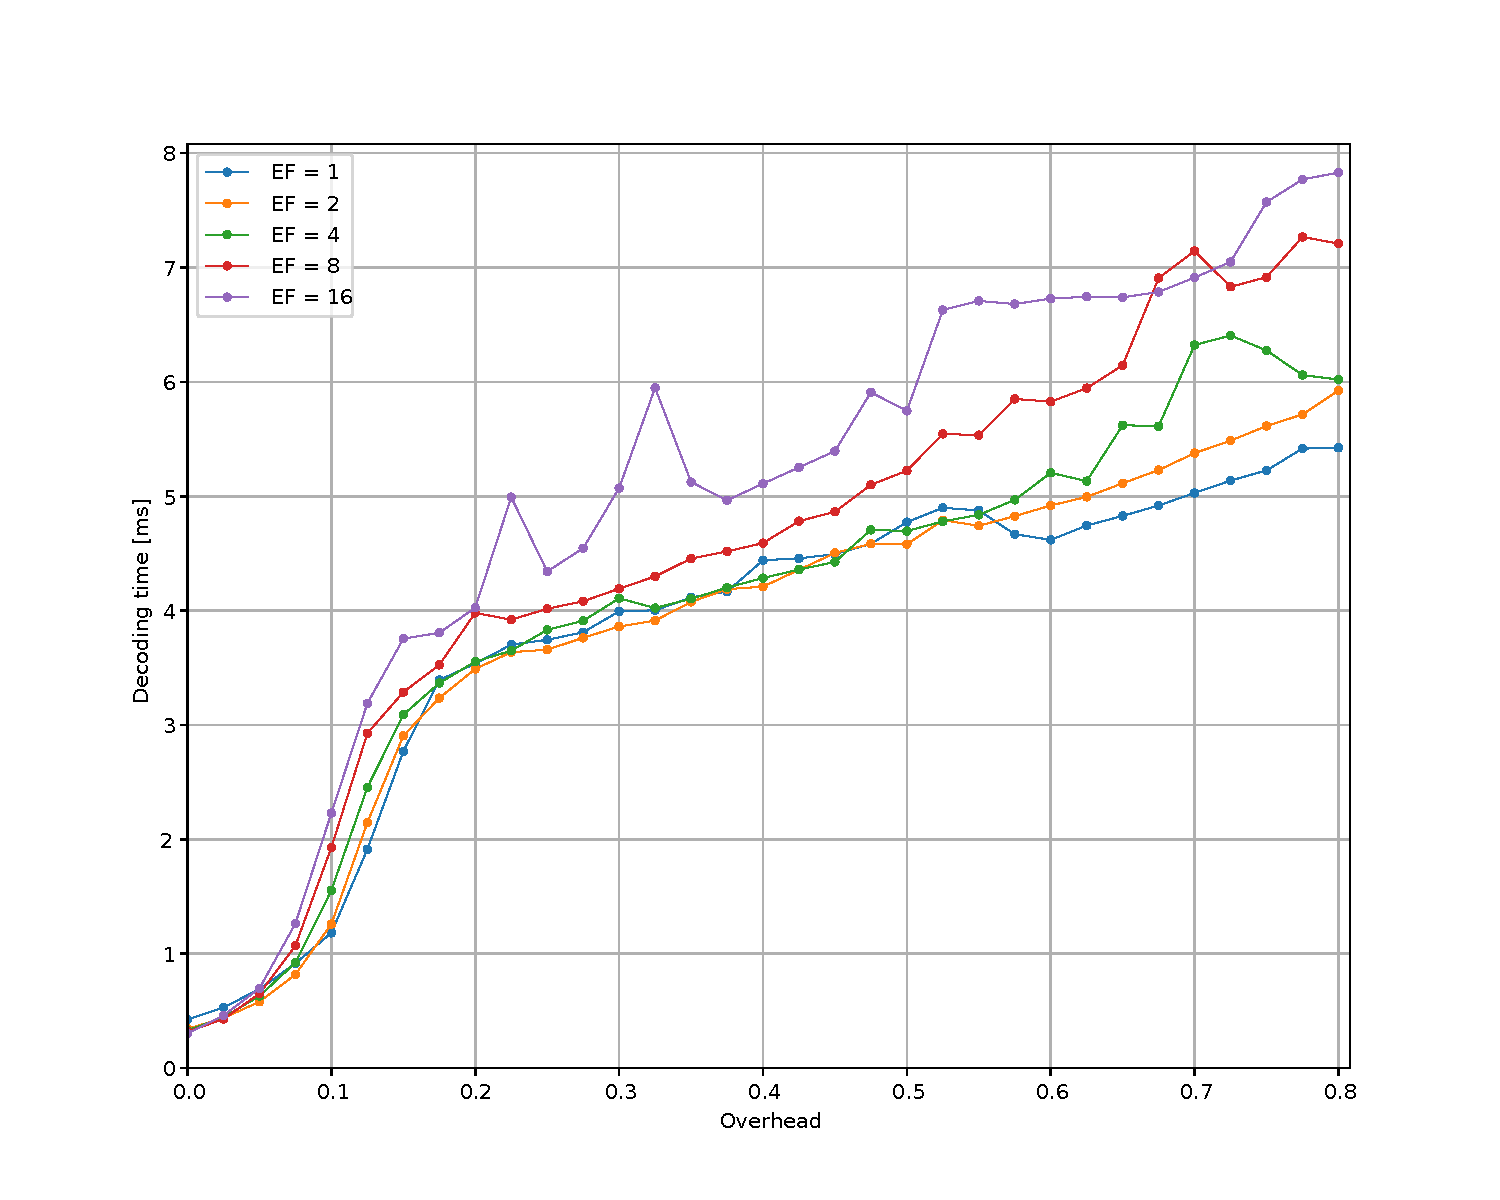
\includegraphics[width=\textwidth]{plot_dec_time_eep}
    \caption{Decodifica EEP}
    \label{fig:dectime_eep}
  \end{subfigure}
  \begin{subfigure}{0.5\textwidth}
    \centering
    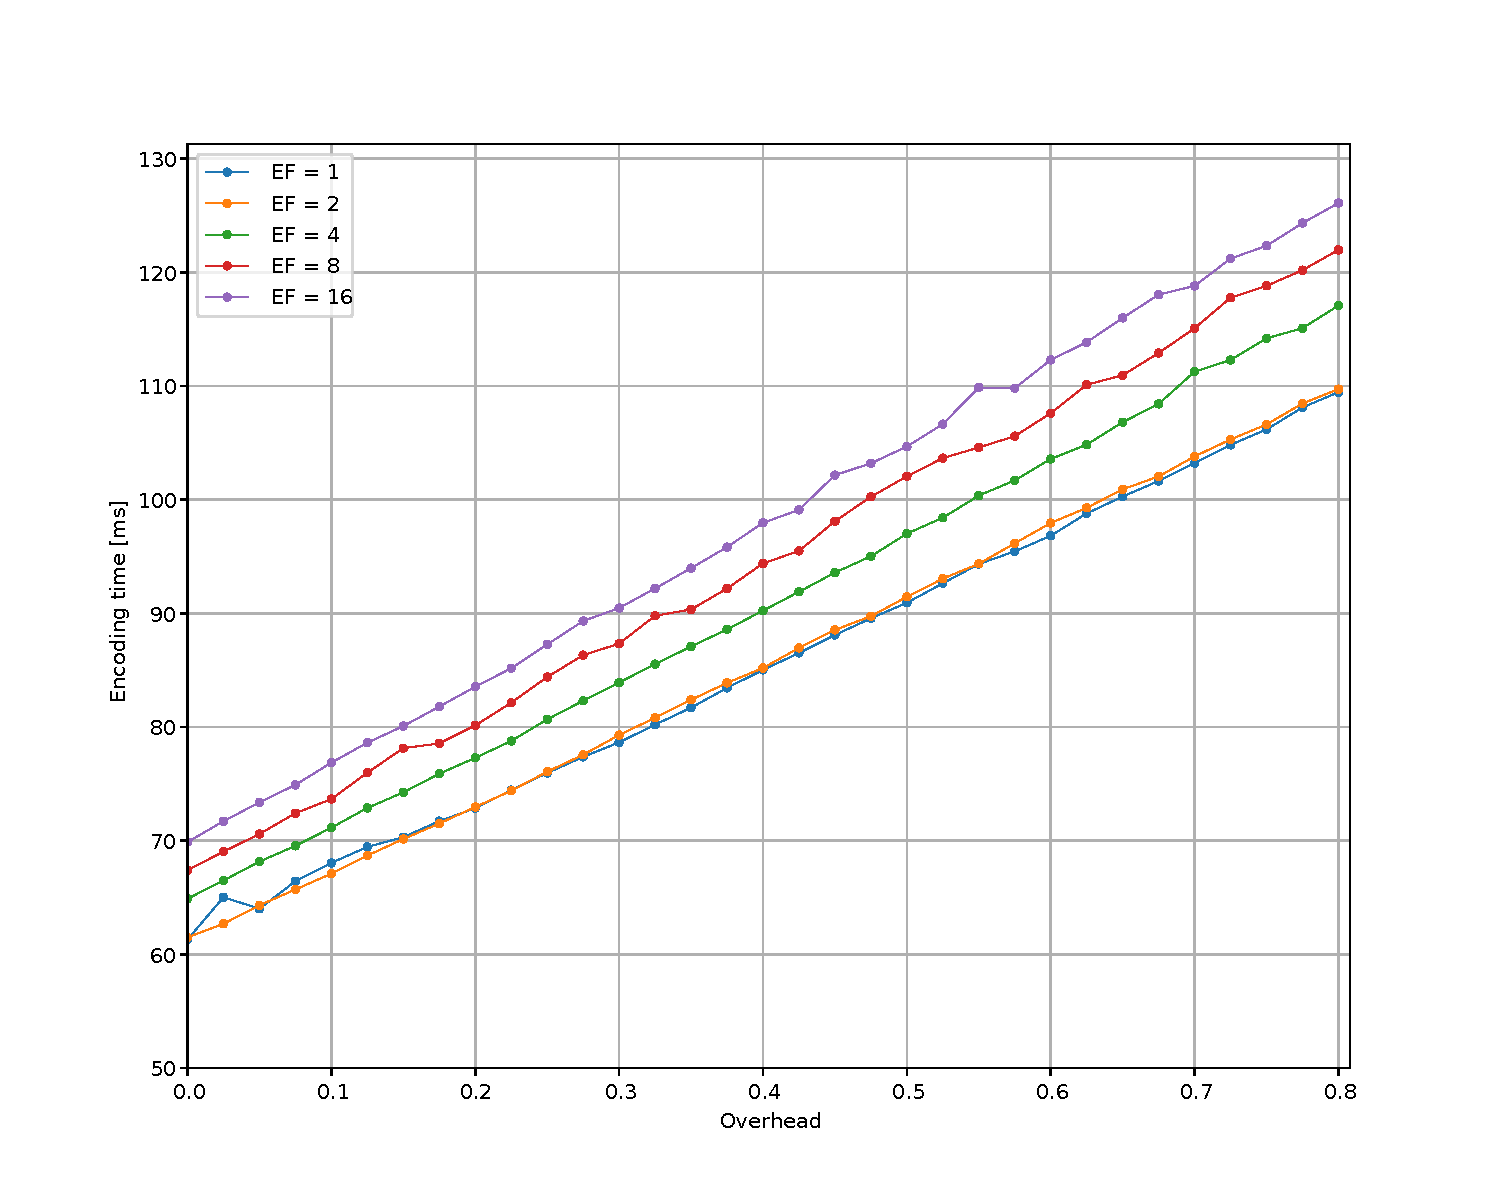
\includegraphics[width=\textwidth]{plot_enc_time_uep}
    \caption{Codifica UEP}
    \label{fig:enctime_uep}
  \end{subfigure}%
  \begin{subfigure}{0.5\textwidth}
    \centering
    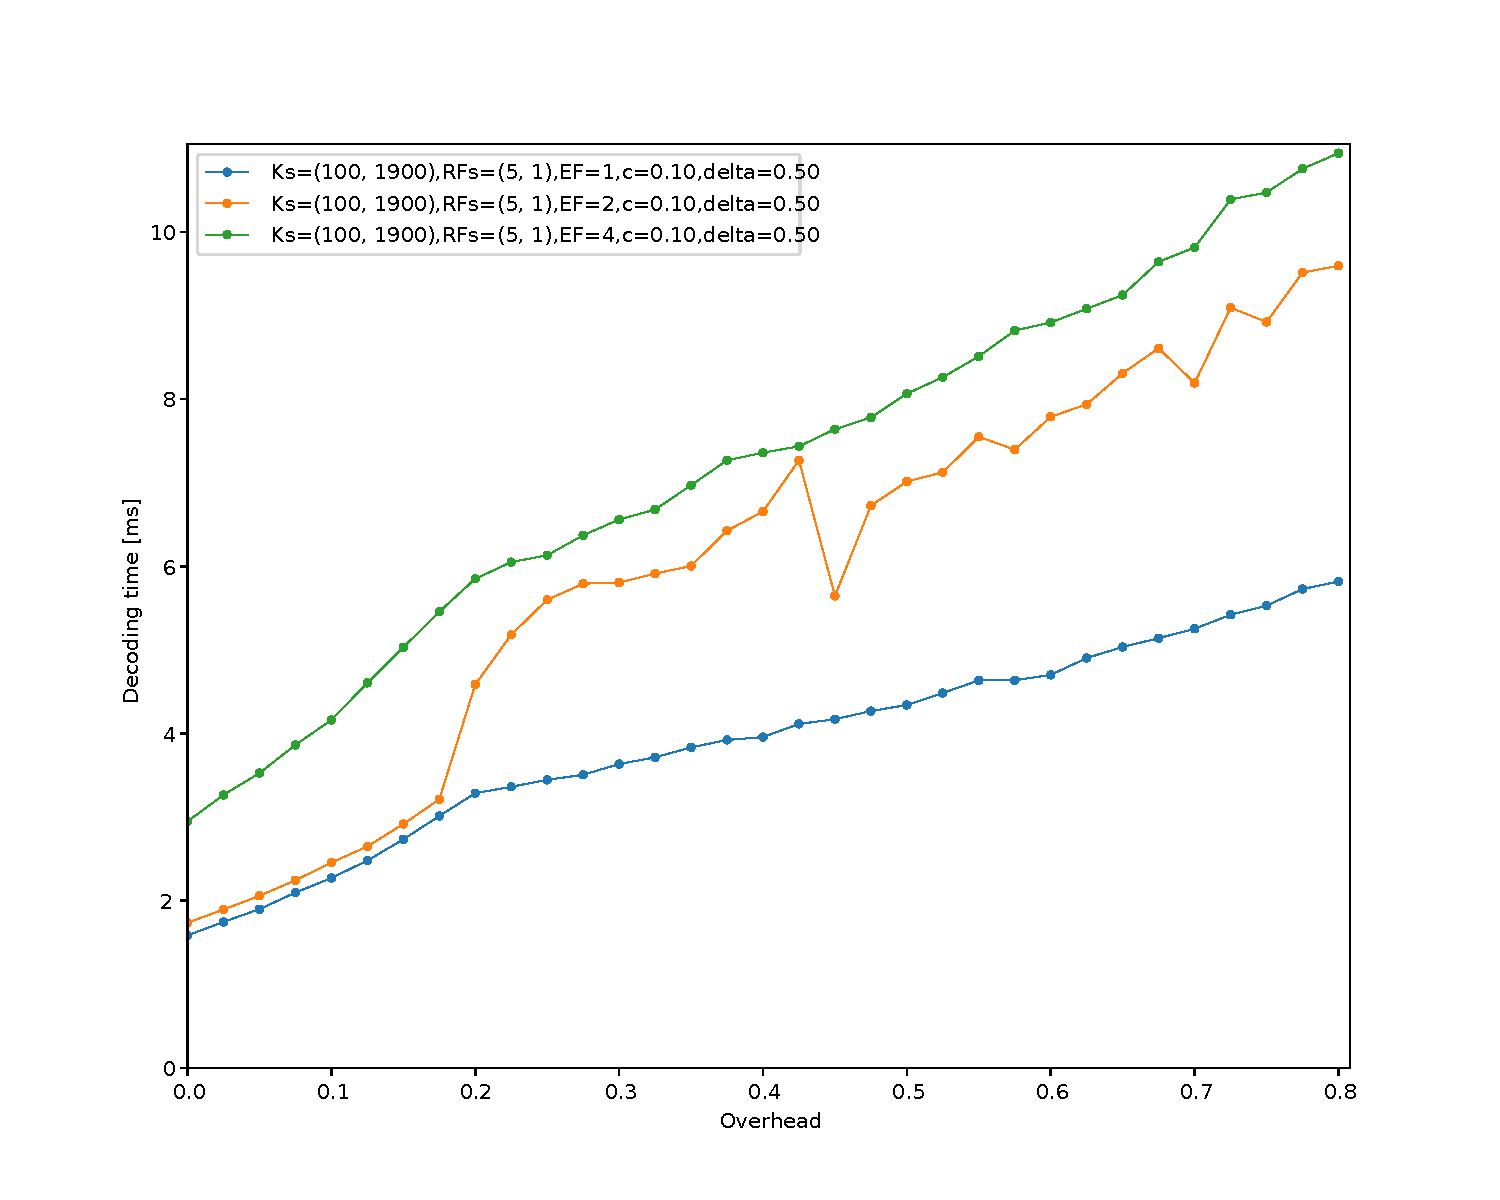
\includegraphics[width=\textwidth]{plot_dec_time_uep}
    \caption{Decodifica UEP}
    \label{fig:dectime_uep}
  \end{subfigure}
  \caption{Tempi medi di codifica e decodifica per un blocco di
    $K=2000$ pacchetti codificato usando EEP o UEP ($K_0 = 100$,
    $RF_0=5$) con $EF \in \{1,2,4\}$.}
  \label{fig:encdec}
\end{figure}
%
Si può vedere che l'andamento è coerente con \cite{uep}: i tempi di
codifica aumentano linearmente al crescere del'overhead e
sub-linearmente al crescere di $EF$; i tempi di decodifica crescono
velocemente fino al livello di overhead in cui la maggior parte dei
pacchetti sono decodificati e, in seguito, la crescita diventa molto
più lenta.
%
I valori dei tempi di decodifica sono dello stesso ordine di grandezza
di quelli riportati in \cite{uep}, mentre i valori dei tempi di
codifica sono molto più alti, sia dell'articolo che dei tempi di
decodifica corrisponenti. Questo può essere spiegato dal fatto che,
mentre l'implementazione del message passing usata nelle simulazioni è
scritta in C++, la generazione dei vettori di codifica è effettuata da
uno script scritto in Python.

\subsection{Scelta della dimensione dei pacchetti}
\label{sec:pktsize}
Il paper \cite{uep} considera simboli di 1 byte durante la codifica,
ma questa scelta non è praticabile nel caso di questa tesina. Il
motivo è dato dall'overhead introdotto aggiungendo degli header a ogni
pacchetto, infatti una dimensione di pacchetto $L=1$ comporterebbe un
overhead del 1500 \% dovuto solo agli header.

Questo overhead decresce all'aumentare della dimensione dei pacchetti
$L$, tuttavia bisogna considerare l'overhead introdotto dalla
segmentazione del video H264.
%
Il video H264 è composto da pacchetti (detti NALU) di dimensioni
variabili che devono essere aggregati o segmentati in pacchetti di
dimensione fissa $L$. Il fatto di considerare due diverse classi di
priorità per le NALU richiede di inserire un certo numero di byte di
padding, ogni volta che termina una sequenza consecutiva di NALU con
la stessa priorità, per ottenere un numero intero di pacchetti di
lunghezza $L$.

Tenendo conto di entrambi questi contributi all'overhead si ottiene il
grafico mostrato in figura~\ref{fig:pktsize} ed è possibile
individuare il valore $L = 388$ che minimizza l'overhead dovuto al
padding e agli header.
% Best packet size = 388
% Min overhead = 0.069367
\begin{figure}[H]
  \centering
  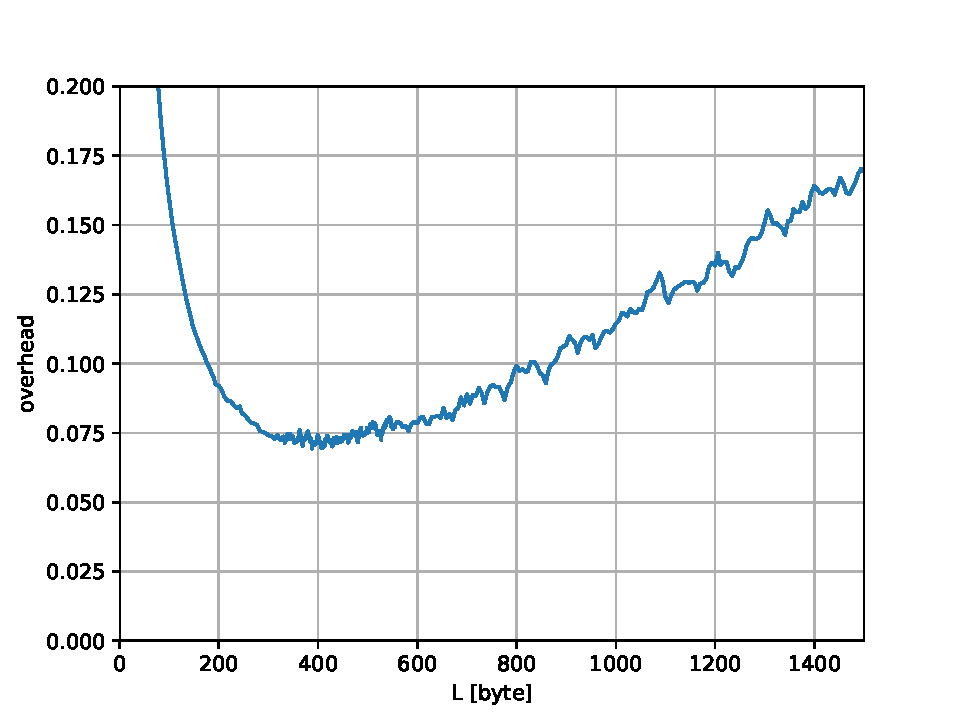
\includegraphics[width=0.8\textwidth]{plot_overhead}
  \caption{Overhead introdotto dalla segmentazione al variare della
    dimensione $L$ dei pacchetti.}
  \label{fig:pktsize}
\end{figure}

\newpage
\section{Conclusioni} % Max 0.5 pages


%\begin{figure}[H]
%	\makebox[\textwidth][c]{\includegraphics[width=16cm]{G10labE_f3.eps}}
%	\caption{Componenti di $\hat{s}$}\label{fig:s2}
%\end{figure}

% Between 3-15 refs
\printbibliography[heading=bibnumbered, title=Bibliografia]
\end{document}